%  LaTeX support: latex@mdpi.com
%  For support, please attach all files needed for compiling as well as the log file, and specify your operating system, LaTeX version, and LaTeX editor.

%=================================================================
% pandoc conditionals added to preserve backwards compatibility with previous versions of rticles

\documentclass[notspecified,article,submit,moreauthors,pdftex]{Definitions/mdpi}


%% Some pieces required from the pandoc template
\setlist[itemize]{leftmargin=*,labelsep=5.8mm}
\setlist[enumerate]{leftmargin=*,labelsep=4.9mm}


%--------------------
% Class Options:
%--------------------

%---------
% article
%---------
% The default type of manuscript is "article", but can be replaced by:
% abstract, addendum, article, book, bookreview, briefreport, casereport, comment, commentary, communication, conferenceproceedings, correction, conferencereport, entry, expressionofconcern, extendedabstract, datadescriptor, editorial, essay, erratum, hypothesis, interestingimage, obituary, opinion, projectreport, reply, retraction, review, perspective, protocol, shortnote, studyprotocol, systematicreview, supfile, technicalnote, viewpoint, guidelines, registeredreport, tutorial
% supfile = supplementary materials

%----------
% submit
%----------
% The class option "submit" will be changed to "accept" by the Editorial Office when the paper is accepted. This will only make changes to the frontpage (e.g., the logo of the journal will get visible), the headings, and the copyright information. Also, line numbering will be removed. Journal info and pagination for accepted papers will also be assigned by the Editorial Office.

%------------------
% moreauthors
%------------------
% If there is only one author the class option oneauthor should be used. Otherwise use the class option moreauthors.

%---------
% pdftex
%---------
% The option pdftex is for use with pdfLaTeX. Remove "pdftex" for (1) compiling with LaTeX & dvi2pdf (if eps figures are used) or for (2) compiling with XeLaTeX.

%=================================================================
% MDPI internal commands - do not modify
\firstpage{1}
\makeatletter
\setcounter{page}{\@firstpage}
\makeatother
\pubvolume{1}
\issuenum{1}
\articlenumber{0}
\pubyear{2023}
\copyrightyear{2023}
%\externaleditor{Academic Editor: Firstname Lastname}
\datereceived{ }
\daterevised{ } % Comment out if no revised date
\dateaccepted{ }
\datepublished{ }
%\datecorrected{} % For corrected papers: "Corrected: XXX" date in the original paper.
%\dateretracted{} % For corrected papers: "Retracted: XXX" date in the original paper.
\hreflink{https://doi.org/} % If needed use \linebreak
%\doinum{}
%\pdfoutput=1 % Uncommented for upload to arXiv.org

%=================================================================
% Add packages and commands here. The following packages are loaded in our class file: fontenc, inputenc, calc, indentfirst, fancyhdr, graphicx, epstopdf, lastpage, ifthen, float, amsmath, amssymb, lineno, setspace, enumitem, mathpazo, booktabs, titlesec, etoolbox, tabto, xcolor, colortbl, soul, multirow, microtype, tikz, totcount, changepage, attrib, upgreek, array, tabularx, pbox, ragged2e, tocloft, marginnote, marginfix, enotez, amsthm, natbib, hyperref, cleveref, scrextend, url, geometry, newfloat, caption, draftwatermark, seqsplit
% cleveref: load \crefname definitions after \begin{document}

%=================================================================
% Please use the following mathematics environments: Theorem, Lemma, Corollary, Proposition, Characterization, Property, Problem, Example, ExamplesandDefinitions, Hypothesis, Remark, Definition, Notation, Assumption
%% For proofs, please use the proof environment (the amsthm package is loaded by the MDPI class).

%=================================================================
% Full title of the paper (Capitalized)
\Title{Trabajo Análisis Exploratorio de Datos}

% MDPI internal command: Title for citation in the left column
\TitleCitation{Trabajo Análisis Exploratorio de Datos}

% Author Orchid ID: enter ID or remove command
%\newcommand{\orcidauthorA}{0000-0000-0000-000X} % Add \orcidA{} behind the author's name
%\newcommand{\orcidauthorB}{0000-0000-0000-000X} % Add \orcidB{} behind the author's name


% Authors, for the paper (add full first names)
\Author{Luis Miguel Rioja Gallo, Anna Cabrerizo
Requena$^{1,2,\ddagger,*}$\href{https://orcid.org/0000-0003-3293-2315}
{\orcidicon}, John Doe$^{2, \dagger, \ddagger}$}


%\longauthorlist{yes}


% MDPI internal command: Authors, for metadata in PDF
\AuthorNames{Luis Miguel Rioja Gallo, Anna Cabrerizo Requena, John Doe}

% MDPI internal command: Authors, for citation in the left column
%\AuthorCitation{Lastname, F.; Lastname, F.; Lastname, F.}
% If this is a Chicago style journal: Lastname, Firstname, Firstname Lastname, and Firstname Lastname.
\AuthorCitation{Leutnant, D.; Doe, J.}

% Affiliations / Addresses (Add [1] after \address if there is only one affiliation.)
\address{%
$^{1}$ \quad Universitat de València - Etse. Burjassot,
València; \href{mailto:ancare2@alumne.uv.es}{\nolinkurl{ancare2@alumne.uv.es}}\\
$^{2}$ \quad Your department Street, City,
Country; \href{mailto:mail@mail.com}{\nolinkurl{mail@mail.com}}\\
}

% Contact information of the corresponding author
\corres{Correspondence: \href{mailto:leutnant@fh-muenster.de}{\nolinkurl{leutnant@fh-muenster.de}};
Tel.: +XX-000-00-0000.}

% Current address and/or shared authorship
\firstnote{Current address: Updated affiliation}
\secondnote{These authors contributed equally to this work.}






% The commands \thirdnote{} till \eighthnote{} are available for further notes

% Simple summary
\simplesumm{A Simple summary goes here.}

%\conference{} % An extended version of a conference paper

% Abstract (Do not insert blank lines, i.e. \\)
\abstract{A single paragraph of about 200 words maximum. For research
articles, abstracts should give a pertinent overview of the work. We
strongly encourage authors to use the following style of structured
abstracts, but without headings: 1) Background: Place the question
addressed in a broad context and highlight the purpose of the study; 2)
Methods: Describe briefly the main methods or treatments applied; 3)
Results: Summarize the article's main findings; and 4) Conclusion:
Indicate the main conclusions or interpretations. The abstract should be
an objective representation of the article, it must not contain results
which are not presented and substantiated in the main text and should
not exaggerate the main conclusions.}


% Keywords
\keyword{keyword 1; keyword 2; keyword 3 (list three to ten pertinent
keywords specific to the article, yet reasonably common within the
subject discipline.).}

% The fields PACS, MSC, and JEL may be left empty or commented out if not applicable
%\PACS{J0101}
%\MSC{}
%\JEL{}

%%%%%%%%%%%%%%%%%%%%%%%%%%%%%%%%%%%%%%%%%%
% Only for the journal Diversity
%\LSID{\url{http://}}

%%%%%%%%%%%%%%%%%%%%%%%%%%%%%%%%%%%%%%%%%%
% Only for the journal Applied Sciences

%%%%%%%%%%%%%%%%%%%%%%%%%%%%%%%%%%%%%%%%%%

%%%%%%%%%%%%%%%%%%%%%%%%%%%%%%%%%%%%%%%%%%
% Only for the journal Data



%%%%%%%%%%%%%%%%%%%%%%%%%%%%%%%%%%%%%%%%%%
% Only for the journal Toxins


%%%%%%%%%%%%%%%%%%%%%%%%%%%%%%%%%%%%%%%%%%
% Only for the journal Encyclopedia


%%%%%%%%%%%%%%%%%%%%%%%%%%%%%%%%%%%%%%%%%%
% Only for the journal Advances in Respiratory Medicine
%\addhighlights{yes}
%\renewcommand{\addhighlights}{%

%\noindent This is an obligatory section in “Advances in Respiratory Medicine”, whose goal is to increase the discoverability and readability of the article via search engines and other scholars. Highlights should not be a copy of the abstract, but a simple text allowing the reader to quickly and simplified find out what the article is about and what can be cited from it. Each of these parts should be devoted up to 2~bullet points.\vspace{3pt}\\
%\textbf{What are the main findings?}
% \begin{itemize}[labelsep=2.5mm,topsep=-3pt]
% \item First bullet.
% \item Second bullet.
% \end{itemize}\vspace{3pt}
%\textbf{What is the implication of the main finding?}
% \begin{itemize}[labelsep=2.5mm,topsep=-3pt]
% \item First bullet.
% \item Second bullet.
% \end{itemize}
%}


%%%%%%%%%%%%%%%%%%%%%%%%%%%%%%%%%%%%%%%%%%

% Pandoc syntax highlighting
\usepackage{color}
\usepackage{fancyvrb}
\newcommand{\VerbBar}{|}
\newcommand{\VERB}{\Verb[commandchars=\\\{\}]}
\DefineVerbatimEnvironment{Highlighting}{Verbatim}{commandchars=\\\{\}}
% Add ',fontsize=\small' for more characters per line
\usepackage{framed}
\definecolor{shadecolor}{RGB}{248,248,248}
\newenvironment{Shaded}{\begin{snugshade}}{\end{snugshade}}
\newcommand{\AlertTok}[1]{\textcolor[rgb]{0.94,0.16,0.16}{#1}}
\newcommand{\AnnotationTok}[1]{\textcolor[rgb]{0.56,0.35,0.01}{\textbf{\textit{#1}}}}
\newcommand{\AttributeTok}[1]{\textcolor[rgb]{0.13,0.29,0.53}{#1}}
\newcommand{\BaseNTok}[1]{\textcolor[rgb]{0.00,0.00,0.81}{#1}}
\newcommand{\BuiltInTok}[1]{#1}
\newcommand{\CharTok}[1]{\textcolor[rgb]{0.31,0.60,0.02}{#1}}
\newcommand{\CommentTok}[1]{\textcolor[rgb]{0.56,0.35,0.01}{\textit{#1}}}
\newcommand{\CommentVarTok}[1]{\textcolor[rgb]{0.56,0.35,0.01}{\textbf{\textit{#1}}}}
\newcommand{\ConstantTok}[1]{\textcolor[rgb]{0.56,0.35,0.01}{#1}}
\newcommand{\ControlFlowTok}[1]{\textcolor[rgb]{0.13,0.29,0.53}{\textbf{#1}}}
\newcommand{\DataTypeTok}[1]{\textcolor[rgb]{0.13,0.29,0.53}{#1}}
\newcommand{\DecValTok}[1]{\textcolor[rgb]{0.00,0.00,0.81}{#1}}
\newcommand{\DocumentationTok}[1]{\textcolor[rgb]{0.56,0.35,0.01}{\textbf{\textit{#1}}}}
\newcommand{\ErrorTok}[1]{\textcolor[rgb]{0.64,0.00,0.00}{\textbf{#1}}}
\newcommand{\ExtensionTok}[1]{#1}
\newcommand{\FloatTok}[1]{\textcolor[rgb]{0.00,0.00,0.81}{#1}}
\newcommand{\FunctionTok}[1]{\textcolor[rgb]{0.13,0.29,0.53}{\textbf{#1}}}
\newcommand{\ImportTok}[1]{#1}
\newcommand{\InformationTok}[1]{\textcolor[rgb]{0.56,0.35,0.01}{\textbf{\textit{#1}}}}
\newcommand{\KeywordTok}[1]{\textcolor[rgb]{0.13,0.29,0.53}{\textbf{#1}}}
\newcommand{\NormalTok}[1]{#1}
\newcommand{\OperatorTok}[1]{\textcolor[rgb]{0.81,0.36,0.00}{\textbf{#1}}}
\newcommand{\OtherTok}[1]{\textcolor[rgb]{0.56,0.35,0.01}{#1}}
\newcommand{\PreprocessorTok}[1]{\textcolor[rgb]{0.56,0.35,0.01}{\textit{#1}}}
\newcommand{\RegionMarkerTok}[1]{#1}
\newcommand{\SpecialCharTok}[1]{\textcolor[rgb]{0.81,0.36,0.00}{\textbf{#1}}}
\newcommand{\SpecialStringTok}[1]{\textcolor[rgb]{0.31,0.60,0.02}{#1}}
\newcommand{\StringTok}[1]{\textcolor[rgb]{0.31,0.60,0.02}{#1}}
\newcommand{\VariableTok}[1]{\textcolor[rgb]{0.00,0.00,0.00}{#1}}
\newcommand{\VerbatimStringTok}[1]{\textcolor[rgb]{0.31,0.60,0.02}{#1}}
\newcommand{\WarningTok}[1]{\textcolor[rgb]{0.56,0.35,0.01}{\textbf{\textit{#1}}}}

% tightlist command for lists without linebreak
\providecommand{\tightlist}{%
  \setlength{\itemsep}{0pt}\setlength{\parskip}{0pt}}

% From pandoc table feature
\usepackage{longtable,booktabs,array}
\usepackage{calc} % for calculating minipage widths
% Correct order of tables after \paragraph or \subparagraph
\usepackage{etoolbox}
\makeatletter
\patchcmd\longtable{\par}{\if@noskipsec\mbox{}\fi\par}{}{}
\makeatother
% Allow footnotes in longtable head/foot
\IfFileExists{footnotehyper.sty}{\usepackage{footnotehyper}}{\usepackage{footnote}}
\makesavenoteenv{longtable}


\usepackage{longtable}
\usepackage{booktabs}
\usepackage{array}
\usepackage{multirow}
\usepackage{wrapfig}
\usepackage{float}
\usepackage{colortbl}
\usepackage{pdflscape}
\usepackage{tabu}
\usepackage{threeparttable}
\usepackage{threeparttablex}
\usepackage[normalem]{ulem}
\usepackage{makecell}
\usepackage{xcolor}

\begin{document}



%%%%%%%%%%%%%%%%%%%%%%%%%%%%%%%%%%%%%%%%%%

\hypertarget{article-header-information}{%
\section{Article Header Information}\label{article-header-information}}

The YAML header includes information needed mainly for formatting the
front and back matter of the article. Required elements include:

\begin{Shaded}
\begin{Highlighting}[]
\FunctionTok{title}\KeywordTok{:}\AttributeTok{ Title of the paper}
\FunctionTok{author}\KeywordTok{:}
\AttributeTok{  }\KeywordTok{{-}}\AttributeTok{ }\FunctionTok{name}\KeywordTok{:}\AttributeTok{ first and last name}
\FunctionTok{    affil}\KeywordTok{: }\CharTok{|}
\NormalTok{      One or more comma seperated numbers corresponding to affilitation}
\NormalTok{      and one or more  comma seperated symbols corresponding }
\NormalTok{      optional notes.}
\AttributeTok{    }\FunctionTok{orcid}\KeywordTok{:}\AttributeTok{ optional orcid number}
\FunctionTok{affiliation}\KeywordTok{:}\AttributeTok{  }
\AttributeTok{  }\KeywordTok{{-}}\AttributeTok{ }\FunctionTok{num}\KeywordTok{:}\AttributeTok{ 1,..., n for each affiliation}
\AttributeTok{    }\FunctionTok{address}\KeywordTok{:}\AttributeTok{ required}
\AttributeTok{    }\FunctionTok{email}\KeywordTok{:}\AttributeTok{ required}
\FunctionTok{authorcitation}\KeywordTok{: }\CharTok{|}
\NormalTok{  Lastname, F.}
\FunctionTok{correspondence}\KeywordTok{: }\CharTok{|}
\NormalTok{  email@email.com; Tel.: +XX{-}000{-}00{-}0000.}
\FunctionTok{journal}\KeywordTok{:}\AttributeTok{ notspecified}
\FunctionTok{type}\KeywordTok{:}\AttributeTok{ article}
\FunctionTok{status}\KeywordTok{:}\AttributeTok{ submit}
\end{Highlighting}
\end{Shaded}

Journal options are in Table \ref{tab:mdpinames}. The \texttt{status}
variable should generally not be changed by authors. The \texttt{type}
variable describes the type of of submission and defaults to
\texttt{article} but can be replaced with any of the ones in Table
\ref{tab:mdpitype}

\begin{table}

\caption{\label{tab:mdpitype}MDPI article types.}
\centering
\begin{tabular}[t]{lll}
\toprule
abstract & entry & retraction\\
addendum & expressionofconcern & review\\
article & extendedabstract & perspective\\
book & datadescriptor & protocol\\
bookreview & editorial & shortnote\\
\addlinespace
briefreport & essay & studyprotocol\\
casereport & erratum & systematicreview\\
comment & hypothesis & supfile\\
commentary & interestingimage & technicalnote\\
communication & obituary & viewpoint\\
\addlinespace
conferenceproceedings & opinion & guidelines\\
correction & projectreport & registeredreport\\
conferencereport & reply & tutorial\\
\bottomrule
\end{tabular}
\end{table}

\hypertarget{journal-specific-yaml-variables}{%
\subsection{Journal Specific YAML
variables}\label{journal-specific-yaml-variables}}

\begin{Shaded}
\begin{Highlighting}[]
\CommentTok{\# for journal Diversity,}
\CommentTok{\# add the Life Science Identifier using:}
\FunctionTok{lsid}\KeywordTok{:}\AttributeTok{ http://zoobank.org/urn:lsid:zoobank.org:act:nnnn}


\CommentTok{\# for journal Applied Sciences}
\CommentTok{\# add featured application}
\FunctionTok{featuredapplication}\KeywordTok{: }\CharTok{|}
\NormalTok{  Authors are encouraged to provide a concise }
\NormalTok{  description of the specific application or }
\NormalTok{  a potential application of the work. This }
\NormalTok{  section is not mandatory.}

\CommentTok{\# for the journal Data}
\CommentTok{\# add dataset doi and license}
\FunctionTok{dataset}\KeywordTok{:}\AttributeTok{ https://doi.org/10.1000/182}
\FunctionTok{datasetlicense}\KeywordTok{:}\AttributeTok{ CC{-}BY{-}4.0}

\CommentTok{\# for the journal Toxins}
\CommentTok{\# add key contributions}
\FunctionTok{keycontributions}\KeywordTok{: }\CharTok{|}
\NormalTok{  The breakthroughs or highlights of the manuscript. }
\NormalTok{  Authors can write one or two sentences to describe }
\NormalTok{  the most important part of the paper.}

\CommentTok{\# for the journal Encyclopedia}
\FunctionTok{encyclopediadef}\KeywordTok{: }\CharTok{|}
\NormalTok{  For entry manuscripts only: please provide a brief overview}
\NormalTok{  of the entry title instead of an abstract.}
\FunctionTok{entrylink}\KeywordTok{:}\AttributeTok{ The Link to this entry published on the encyclopedia platform.}

\CommentTok{\# for the journal Advances in Respiratory Medicine}
\CommentTok{\# add highlights}
\FunctionTok{addhighlights}\KeywordTok{: }\CharTok{|}
\NormalTok{  This is an obligatory section in “Advances in Respiratory Medicine”, }
\NormalTok{  whose goal is to increase the discoverability and readability of the}
\NormalTok{  article via search engines and other scholars. Highlights should not }
\NormalTok{  be a copy of the abstract, but a simple text allowing the reader to }
\NormalTok{  quickly and simplified find out what the article is about and what can }
\NormalTok{  be cited from it. Each of these parts should be devoted up to 2\textasciitilde{}bullet }
\NormalTok{  points.}
\end{Highlighting}
\end{Shaded}

\startlandscape

\begin{longtable}[t]{llllllll}
\caption{\label{tab:mdpinames}MDPI journal names.}\\
\toprule
agriculture & air & biologics & clinpract & dairy & ecologies & gases & NOx\_HH\\
agriengineering & algorithms & biology & clockssleep & data & education & C6H6 & O3\_HH\\
agrochemicals & atmosphere & biophysica & cmd & ddc & environments & CO\_HH & PM10\\
agronomy & biochem & carbon & covid & earth & environsciproc & NO\_HH & PM25\\
ai & bioengineering & climate & crops & ebj & epidemiologia & N02\_HH & S02\_HH\\
\bottomrule
\end{longtable}
\finishlandscape

\hypertarget{introducciuxf3n}{%
\section{Introducción}\label{introducciuxf3n}}

Dentro del marco del Plan Nacional del Instituto Nacional de Estadística
(INE) se encuentra el Estudio Estadístico para la Evaluación de la
Calidad del Aire, además cuenta con un visor en tiempo real que
determina el Índice de Calidad del Aire (ICA) de toda España.

El ICA clasifica la calidad del aire en 6 categorías: buena,
razonablemente buena, regular, desfavorable, muy desfavorable y
extremadamente desfavorable. A cada estación se le asigna la categoría
más baja en términos de calidad del aire considerando cualquier
contaminante que se evalúe. Los contaminantes incluidos en el índice son
las Partículas en Suspensión (PM10), Partículas en Suspensión más finas
(PM2,5), Ozono Troposférico (O3), Dióxido de Nitrógeno (NO2) y Dióxido
de Azufre (SO2).

Todo lo relacionado con el cálculo y límites establecidos del ICA se
encuentra legislado por la Resolución del 2 de septiembre de 2020, de la
Dirección General de Calidad y Evaluación Ambiental, por la que se
modifica el Anexo de la Orden TEC/351/2019, de 18 de marzo, y por la que
se aprueba el Índice Nacional de Calidad del Aire. Esta resolución
incluye un anexo con la metodología para el cálculo del ICA.

\hypertarget{procesamiento-de-datos}{%
\section{Procesamiento de Datos}\label{procesamiento-de-datos}}

Este trabajo se centra en el procesamiento de datos en el ámbito del
análisis de la calidad del aire, abordando un conjunto de datos
recopilados durante los años 2018-2022. Inicialmente, el dataset
presentaba desafíos inherentes, como la presencia de valores faltantes y
una estructura no tidy. La tarea principal consistió en transformar esta
información en un formato ``tidy'' para garantizar la coherencia de los
datos.

Con un total de nueve archivos CSV por año que detallan parámetros de
mediciones horarias del aire, así como, un archivo de metadatos de cada
año con información relevante sobre las estaciones, el dataset depurado
establece una base sólida para análisis estadísticos univariantes y
bivariantes que nos permitirán abordar el estudio del ICA en los últimos
cinco años en la Comunidad Autónoma de Valencia. Por lo que se establece
como objetivo en el procesamiento de los datos el compilar la mayor
información posible para poder obtener el ICA como variable categórica y
sacar conclusiones.

\hypertarget{formato-tidy}{%
\section{Formato tidy}\label{formato-tidy}}

En un primer paso, emprendemos la tarea de obtener un conjunto de datos
consolidado a partir de nuestros registros. Este proceso implica un
análisis detallado de cada año, con el objetivo de integrar las columnas
correspondientes a las observaciones diarias de diversos agentes
químicos del aire presentes en cada hoja de Excel. En concreto,
disponemos de medidas de Partículas en suspensión (PM10 y PM2,5), Ozono
troposférico (O3), Dióxido de nitrógeno (NO2), Dióxido de azufre (SO2),
Benzeno (C6H6), Monóxido de Carbono (CO), Monóxido de Nitrógeno (NO) y
Óxidos de Nitrógeno (NOx), cada una de las variables en un CSV
diferente. La finalidad es fusionar estas columnas en una única entidad
independiente que contenga todas las observaciones de dicho parámetro
durante los cinco años contemplados en el estudio, además de añadirle
más variables procedentes de los metadatos de las estaciones.

Este enfoque permite la generación de un conjunto de datos estructurado
de manera ``tidy'', donde cada variable se representa en una columna
individual y cada observación de una variable ocupa una fila
independiente. La consolidación de las diversas tablas y CSV se lleva a
cabo considerando las variables comunes, es decir, los parámetros del
aire analizados. Como resultado, nuestro nuevo dataset presenta una
primera fila que contiene los nombres representativos de las variables,
estableciendo así un marco coherente para el análisis subsiguiente.

Cada archivo se encuentra estructurado originalmente de la siguiente
manera:

\begin{tabular}{r|r|r|r|l|r|r|r|r|r|r|r|r|r|r|r|r|r|r|r|r|r|r|r|r|r|r|r|r|r|r|r}
\hline
PROVINCIA & MUNICIPIO & ESTACION & MAGNITUD & PUNTO\_MUESTREO & ANNO & MES & DIA & H01 & H02 & H03 & H04 & H05 & H06 & H07 & H08 & H09 & H10 & H11 & H12 & H13 & H14 & H15 & H16 & H17 & H18 & H19 & H20 & H21 & H22 & H23 & H24\\
\hline
1 & 22 & 1 & 8 & 01022001\_8\_8 & 2018 & 1 & 1 & 2 & 0 & 0 & 0 & 0 & 1 & 0 & 0 & 0 & 0 & NA & 2 & 2 & 1 & 2 & 3 & 3 & 3 & 4 & 3 & 3 & 3 & 3 & 2\\
\hline
1 & 22 & 1 & 8 & 01022001\_8\_8 & 2018 & 1 & 2 & 2 & 3 & 1 & 1 & 1 & 1 & 2 & 3 & 3 & 3 & 3 & 4 & 4 & 3 & 3 & 3 & 3 & 4 & 2 & 4 & 3 & 3 & 3 & 3\\
\hline
1 & 22 & 1 & 8 & 01022001\_8\_8 & 2018 & 1 & 3 & 1 & 1 & 1 & 1 & 1 & 1 & 2 & 3 & 3 & 3 & 4 & 1 & 3 & 5 & 4 & 5 & 5 & 5 & 5 & 5 & 5 & 5 & 5 & 4\\
\hline
1 & 22 & 1 & 8 & 01022001\_8\_8 & 2018 & 1 & 4 & 3 & 3 & 2 & 2 & 2 & 1 & 2 & 3 & 3 & 3 & 3 & 2 & 1 & 2 & 1 & 3 & 3 & 3 & 3 & 3 & 3 & 3 & 3 & 2\\
\hline
1 & 22 & 1 & 8 & 01022001\_8\_8 & 2018 & 1 & 5 & 1 & 1 & 1 & 1 & 1 & 1 & 1 & 4 & 4 & 5 & 6 & 5 & 5 & 6 & 6 & 5 & 4 & 5 & 9 & 12 & 10 & 6 & 3 & 3\\
\hline
1 & 22 & 1 & 8 & 01022001\_8\_8 & 2018 & 1 & 11 & 2 & 1 & 0 & 0 & 0 & 1 & 2 & 4 & 5 & 4 & 5 & 5 & 5 & 5 & 5 & 5 & 7 & 6 & 6 & 5 & 7 & 9 & 6 & 4\\
\hline
\end{tabular}

En la que cada observación corresponde a la medición de las diferentes
estaciones de medida de toda España, por lo que inicialmente se filtran
los valores a los correspondientes a la CA de Valencia y se restructura
para conseguir el valor de la variable en una única columna a lo largo
del tiempo.Al ser datos horarios, y para poder establecer diariamente el
peor ICA obtenido, se decide computar el valor de la variable como el
máximo medido en 24 horas.

Una vez cargados los dataset, se unen entre ellos para obtener un
conjunto de datos en el que las variables estan repartidas en cada
columna:

\begin{tabular}{l|r|r|r|r|r|r|r|r|r|r|r}
\hline
Fecha & MUNICIPIO & PROVINCIA & ESTACION & C6H6.num & CO.num & NO2.num & NOx.num & O3.num & PM10.num & PM25.num & SO2.num\\
\hline
2022-01-01 & 5 & 12 & 5 & NA & 0.1 & 26 & NA & 63 & 34 & 9 & NA\\
\hline
2022-01-01 & 9 & 3 & 6 & NA & 0.1 & 22 & NA & 60 & NA & NA & 11\\
\hline
2022-01-01 & 9 & 12 & 7 & NA & 0.2 & 46 & NA & 58 & 46 & 46 & 6\\
\hline
2022-01-01 & 10 & 46 & 1 & NA & 0.2 & 15 & NA & 48 & 8 & 8 & 4\\
\hline
2022-01-01 & 14 & 3 & 6 & 2.1 & 0.5 & 64 & NA & 72 & NA & NA & 4\\
\hline
2022-01-01 & 14 & 3 & 8 & NA & NA & 61 & NA & 72 & NA & NA & 3\\
\hline
\end{tabular}

Posteriormente se cargan los metadatos correspondientes a cada año y
añadimos las variables de Tipo de Área (Urbana, Suburbana y Rural),
Latitud y Longitud de la estación de medida, y los nombres del Municipio
y Provincia donde se encuentran.

\begin{tabular}{l|l|r|r|l|l|r|r|r|r|r|r|r|r|r|r}
\hline
N\_PROVINCIA & N\_MUNICIPIO & LATITUD\_G & LONGITUD\_G & TIPO\_AREA & Fecha & ESTACION & C6H6.num & CO.num & NO.num & NO2.num & NOx.num & O3.num & PM10.num & PM25.num & SO2.num\\
\hline
CASTELLÓN/CASTELLÓ & TORRE ENDOMÉNECH & 40.26944 & -0.07889 & RURAL & 2018-07-29 & 1 & NA & NA & NA & NA & NA & 98 & NA & NA & NA\\
\hline
CASTELLÓN/CASTELLÓ & TORRE ENDOMÉNECH & 40.26944 & -0.07889 & RURAL & 2018-02-15 & 1 & NA & NA & NA & NA & NA & 68 & NA & NA & NA\\
\hline
CASTELLÓN/CASTELLÓ & TORRE ENDOMÉNECH & 40.26944 & -0.07889 & RURAL & 2018-11-14 & 1 & NA & NA & NA & NA & NA & 89 & NA & NA & NA\\
\hline
CASTELLÓN/CASTELLÓ & TORRE ENDOMÉNECH & 40.26944 & -0.07889 & RURAL & 2018-08-02 & 1 & NA & NA & NA & NA & NA & 99 & NA & NA & NA\\
\hline
CASTELLÓN/CASTELLÓ & TORRE ENDOMÉNECH & 40.26944 & -0.07889 & RURAL & 2018-11-24 & 1 & NA & NA & NA & NA & NA & 84 & NA & NA & NA\\
\hline
CASTELLÓN/CASTELLÓ & TORRE ENDOMÉNECH & 40.26944 & -0.07889 & RURAL & 2018-08-27 & 1 & NA & NA & NA & NA & NA & 84 & NA & NA & NA\\
\hline
\end{tabular}

En un primer análisis rápido de las variables observamos una gran
cantidad de valores perdidos,

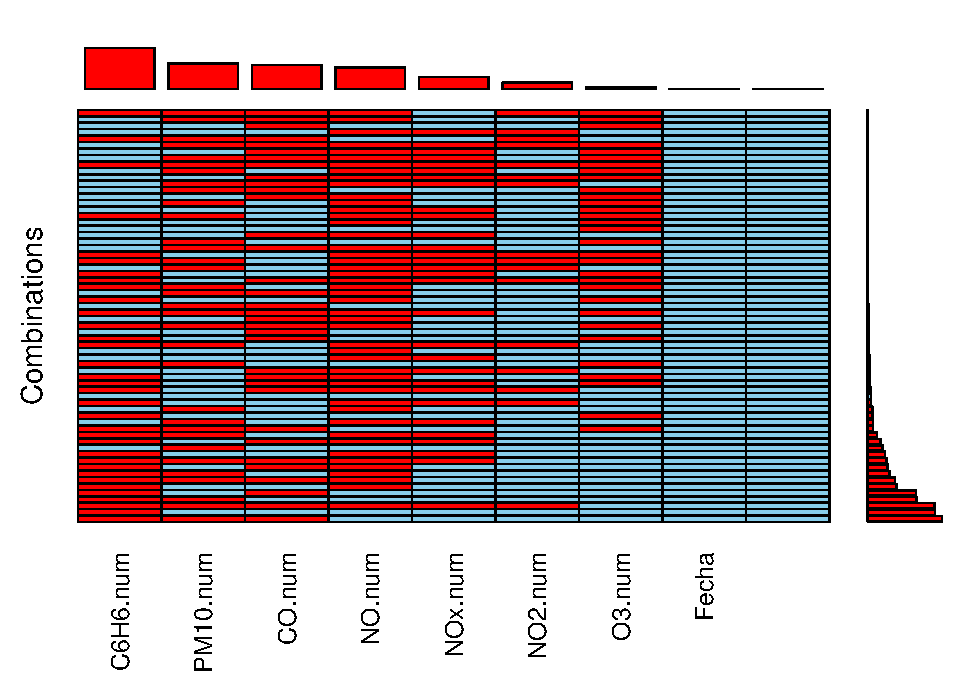
\includegraphics{ProyectoAED2023_files/figure-latex/unnamed-chunk-5-1.pdf}

\begin{verbatim}
## 
##  Variables sorted by number of missings: 
##  Variable Count
##  C6H6.num 91293
##  PM10.num 56927
##    CO.num 53920
##    NO.num 47859
##   NOx.num 27331
##   NO2.num 14397
##    O3.num  4311
##     Fecha     0
##  ESTACION     0
\end{verbatim}

esto es debido a que no en todas las estaciones se miden las mismas
variables, para solucionar esto, lo establecido en la metodología es
usar el valor de la estación más próxima, por ello y para preparar los
datos, se transforma la latitud y longitud a coordenadas proyectadas, de
esta manera nos garantizamos poder usar distancias euclideas en caso de
imputación por proximidad, además se pasan las fecha a días desde el
01-01-2018, que es la fecha de la primera observación de nuestro
conjunto, para establecer una tercera dimensión de proximidad en tiempo.
Por último se categoriza la variable de Tipo de Area donde se encuentra
la estación.

\hypertarget{limpieza-de-datos}{%
\section{Limpieza de datos}\label{limpieza-de-datos}}

Una vez adquirido un conjunto de datos organizado en formato tidy, es
necesario llevar a cabo un proceso de limpieza. Este procedimiento
implica la evaluación minuciosa de cada inconsistencia, tales como los
valores faltantes (NAs) y los valores atípicos (outliers). Con el
propósito de abordar estas discrepancias, se implementan diversos
procedimientos y técnicas especializadas.

\hypertarget{outliers-revisar-esto-la-regla-del-3-sigma-es-para-distribuciones-gaussianas-yo-la-quitaba}{%
\subsection{Outliers (revisar esto, la regla del 3 sigma es para
distribuciones gaussianas, yo la
quitaba)}\label{outliers-revisar-esto-la-regla-del-3-sigma-es-para-distribuciones-gaussianas-yo-la-quitaba}}

Como es ampliamente conocido, un ``outlier'' se define como un valor
atípico en un conjunto de datos que exhibe una marcada disparidad con
respecto al resto de las observaciones. Para analizar la presencia de
tales observaciones atípicas, se emplean tres técnicas específicas: la
regla de 3 sigma, la regla de Hampel, la regla de boxplot y la regla de
los percentiles. Obtuvimos la siguiente tabla:

Aquí utilizamos los códigos implementados anteriormente en cada una de
las variables numéricas para detectar los outliers

\begin{verbatim}
## # A tibble: 6 x 5
##   Chemical_Element `3-Sigma`   IQR Hampel Percentil
##   <chr>                <int> <int>  <int>     <int>
## 1 NO2.num                803  1789    301       709
## 2 NOx.num                725  1379   1658      6215
## 3 O3.num                 789  2191   2169      7247
## 4 PM10.num              1750  8298    353      2435
## 5 PM25.num              2336 10336   6661      6048
## 6 SO2.num               8916  3644   3496      3768
\end{verbatim}

En esta tabla visualizamos un recuento de la cantidad de outliers
detectados con cada método.

Ahora bien, tenemos que analizar que consideramos un valor atípico en
nuestro caso. Para ello, debemos establecer algún criterio. Después de
documentarnos, encontramos en el BOE (Boletín oficial del Estado) la
siguiente tabla:

\begin{longtable}[]{@{}
  >{\raggedright\arraybackslash}p{(\columnwidth - 10\tabcolsep) * \real{0.1379}}
  >{\raggedright\arraybackslash}p{(\columnwidth - 10\tabcolsep) * \real{0.1207}}
  >{\raggedright\arraybackslash}p{(\columnwidth - 10\tabcolsep) * \real{0.1034}}
  >{\raggedright\arraybackslash}p{(\columnwidth - 10\tabcolsep) * \real{0.1207}}
  >{\raggedright\arraybackslash}p{(\columnwidth - 10\tabcolsep) * \real{0.1379}}
  >{\raggedright\arraybackslash}p{(\columnwidth - 10\tabcolsep) * \real{0.3793}}@{}}
\toprule\noalign{}
\begin{minipage}[b]{\linewidth}\raggedright
\(S0_{2}\)
\end{minipage} & \begin{minipage}[b]{\linewidth}\raggedright
PM2,5
\end{minipage} & \begin{minipage}[b]{\linewidth}\raggedright
PM10
\end{minipage} & \begin{minipage}[b]{\linewidth}\raggedright
\(O_{3}\)
\end{minipage} & \begin{minipage}[b]{\linewidth}\raggedright
\(NO_{2}\)
\end{minipage} & \begin{minipage}[b]{\linewidth}\raggedright
CATEGORÍA DEL ÍNDICE
\end{minipage} \\
\midrule\noalign{}
\endhead
\bottomrule\noalign{}
\endlastfoot
751-1250 & 76-800 & 151-1200 & 381-800 & 341-1000 & Extremadamente
Desfavorable \\
\end{longtable}

Para utilizar la detección de valores atípicos y asignarles esta
categoría, en nuestro caso calculamos tanto el valor máximo como el
mínimo para cada uno de los parámetros químicos. Este proceso nos
permite evaluar si dichos valores caen fuera del rango establecido en la
tabla anterior, lo que justificaría su clasificación como outliers. Tras
realizar estos cálculos, hemos verificado que los valores identificados
como outliers son válidos y, por ende, hemos decidido mantenerlos en el
conjunto de datos.

\hypertarget{imputaciuxf3n-nas}{%
\subsection{Imputación NAs}\label{imputaciuxf3n-nas}}

El siguiente paso en el proceso de limpieza de nuestro conjunto de datos
implica la imputación de los valores faltantes, comúnmente conocidos
como NAs. Para abordar esta tarea, hemos estudiado diversas técnicas en
clase, entre las cuales se incluyen: la eliminación de datos, la
imputación con un valor estimado basado en los valores conocidos, la
imputación mediante un modelo predictivo o la imputación al valor más
cercano utilizando el algoritmo KNN (k-vecinos más cercanos).

Para ello se realiza un análisis preliminar de los datos, calculando las
correlaciones entre variables.

A pesar de que el ICA solo usa 5 de las 9 variables que disponemmos, se
ha decidido dejarlas inicialmente por si exsite alguna relación que las
conviertan en posibles predictores de datos faltantes, por lo que
analizamos las covarianzas y correlaciones entre ellos,

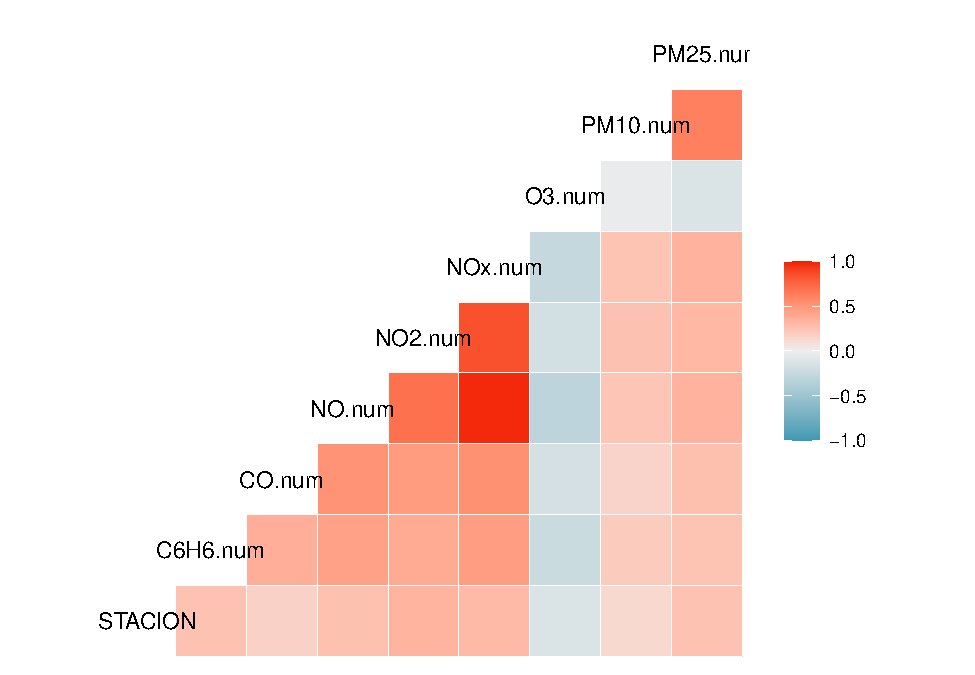
\includegraphics{ProyectoAED2023_files/figure-latex/unnamed-chunk-12-1.pdf}

\begin{tabular}{l|r|r|r|r|r|r|r|r|r}
\hline
  & ESTACION & C6H6.num & CO.num & NO.num & NO2.num & NOx.num & O3.num & PM10.num & PM25.num\\
\hline
ESTACION & 0 & 0.000000 & 0.0000000 & 0.000000 & 0.00000 & 0.00000 & 0.000000 & 0.000000 & 0.0000000\\
\hline
C6H6.num & 0 & 24.729670 & 0.5724250 & 152.218391 & 63.75446 & 289.77848 & -42.419587 & 47.900037 & 29.5360571\\
\hline
CO.num & 0 & 0.572425 & 0.0489320 & 7.127909 & 3.30182 & 14.00281 & -1.905907 & 2.019528 & 0.9951127\\
\hline
NO.num & 0 & 152.218391 & 7.1279094 & 2528.283413 & 882.25600 & 4661.00488 & -619.266677 & 501.070818 & 297.5710857\\
\hline
NO2.num & 0 & 63.754455 & 3.3018198 & 882.255998 & 532.65585 & 1834.45137 & -188.779011 & 287.428304 & 158.7820322\\
\hline
NOx.num & 0 & 289.778482 & 14.0028126 & 4661.004883 & 1834.45137 & 8825.49803 & -1095.762364 & 1030.169405 & 591.3633680\\
\hline
O3.num & 0 & -42.419587 & -1.9059066 & -619.266677 & -188.77901 & -1095.76236 & 511.685364 & -45.327732 & -38.3192311\\
\hline
PM10.num & 0 & 47.900037 & 2.0195275 & 501.070818 & 287.42830 & 1030.16941 & -45.327732 & 600.269287 & 243.9767201\\
\hline
PM25.num & 0 & 29.536057 & 0.9951127 & 297.571086 & 158.78203 & 591.36337 & -38.319231 & 243.976720 & 180.3501367\\
\hline
\end{tabular}

observandose una fuerte correlación entre los Óxidos Nitroso.

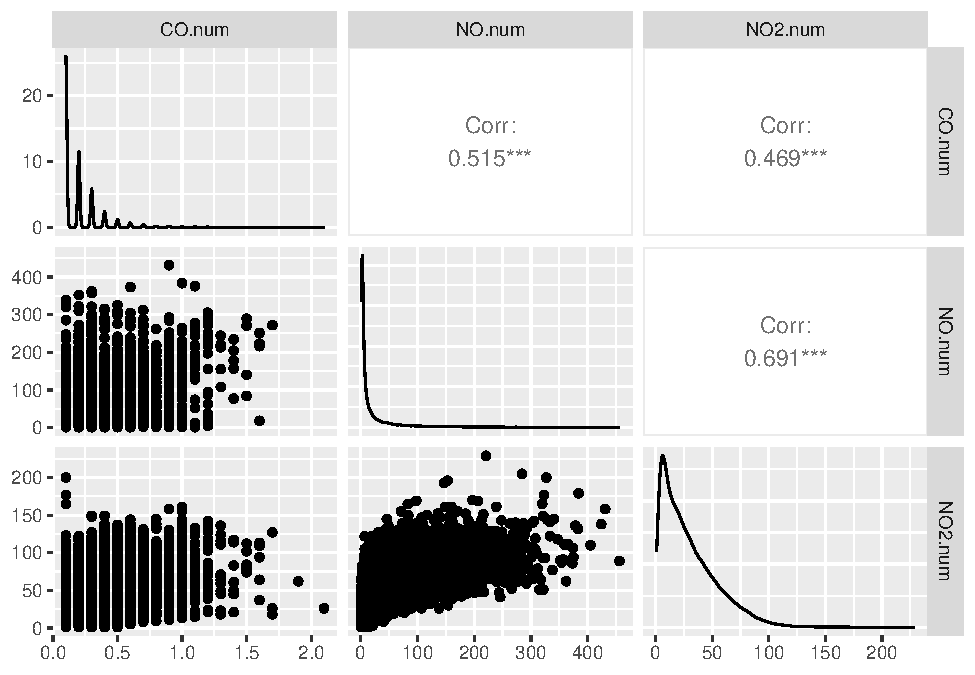
\includegraphics{ProyectoAED2023_files/figure-latex/unnamed-chunk-13-1.pdf}

y decidiendose usar las variables NO y NOx para inferir los datos
faltantes del NO2, compuesto necesario para calcular el ICA.

Tras analizar los datos de NOx y NO se observa que no existen datos en
los años 2021 y 2022 por lo que se acota la posibilidad de inferencia
del 2018 al 2020.

De manera que se entrena un modelo lineal múltiple con los siguientes
resultados para el conjunto de test:

\begin{verbatim}
## 
## Call:
## lm(formula = NO2.num ~ NOx.num + NO.num, data = train)
## 
## Residuals:
##      Min       1Q   Median       3Q      Max 
## -300.316   -1.748   -0.896    0.560   89.341 
## 
## Coefficients:
##              Estimate Std. Error t value Pr(>|t|)    
## (Intercept)  1.810047   0.042584   42.51   <2e-16 ***
## NOx.num      0.973668   0.001452  670.76   <2e-16 ***
## NO.num      -1.438813   0.002968 -484.70   <2e-16 ***
## ---
## Signif. codes:  0 '***' 0.001 '**' 0.01 '*' 0.05 '.' 0.1 ' ' 1
## 
## Residual standard error: 5.236 on 40405 degrees of freedom
##   (6670 observations deleted due to missingness)
## Multiple R-squared:  0.9569, Adjusted R-squared:  0.9568 
## F-statistic: 4.48e+05 on 2 and 40405 DF,  p-value: < 2.2e-16
\end{verbatim}

\begin{verbatim}
## RMSE con el conjunto de test=  4.807143
\end{verbatim}

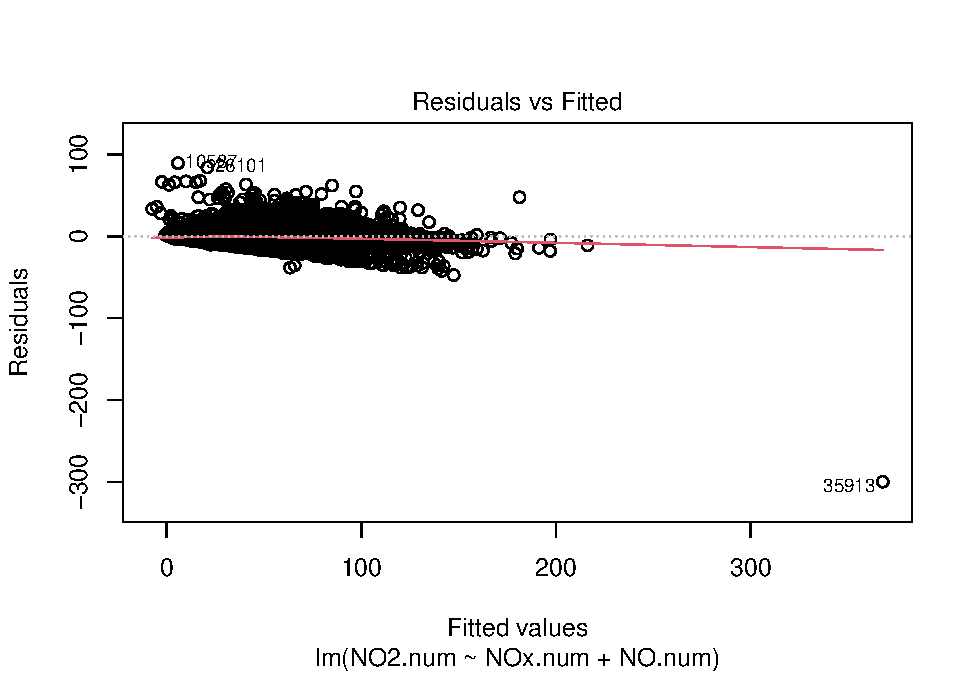
\includegraphics{ProyectoAED2023_files/figure-latex/unnamed-chunk-14-1.pdf}
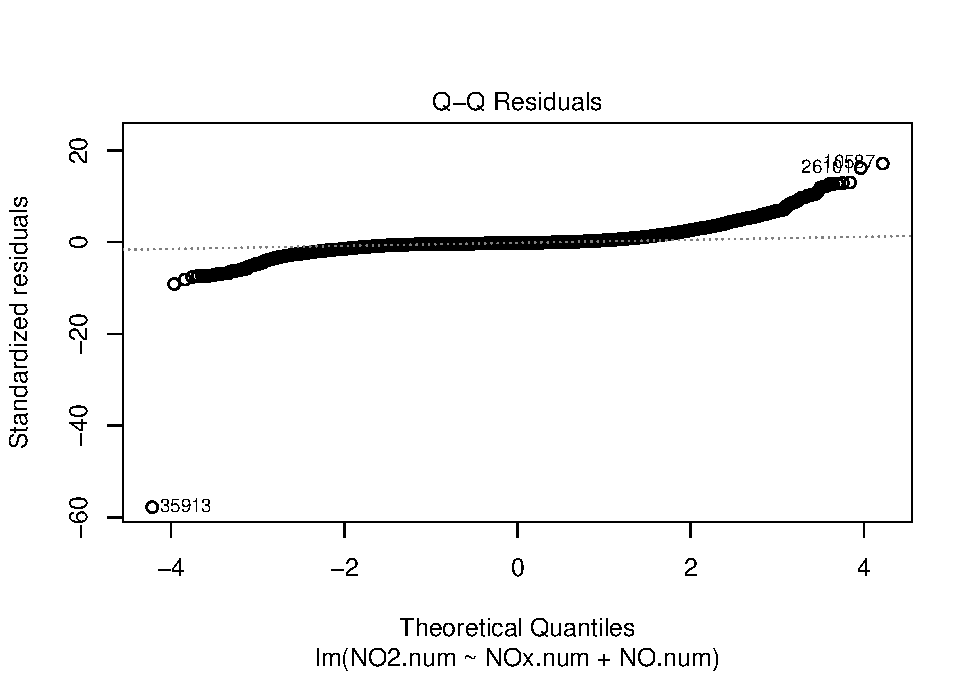
\includegraphics{ProyectoAED2023_files/figure-latex/unnamed-chunk-14-2.pdf}
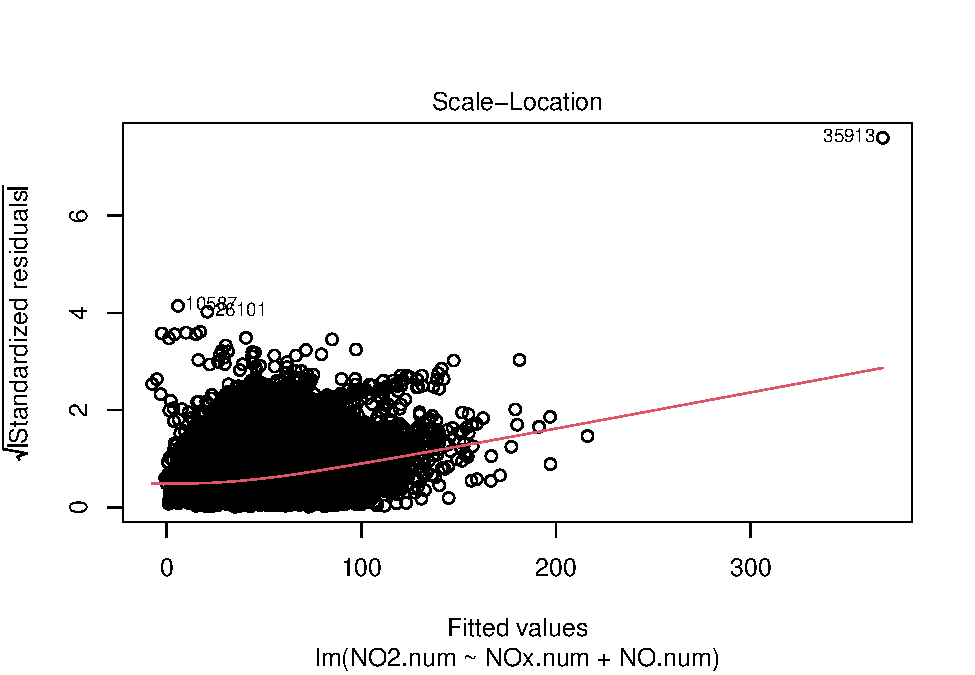
\includegraphics{ProyectoAED2023_files/figure-latex/unnamed-chunk-14-3.pdf}
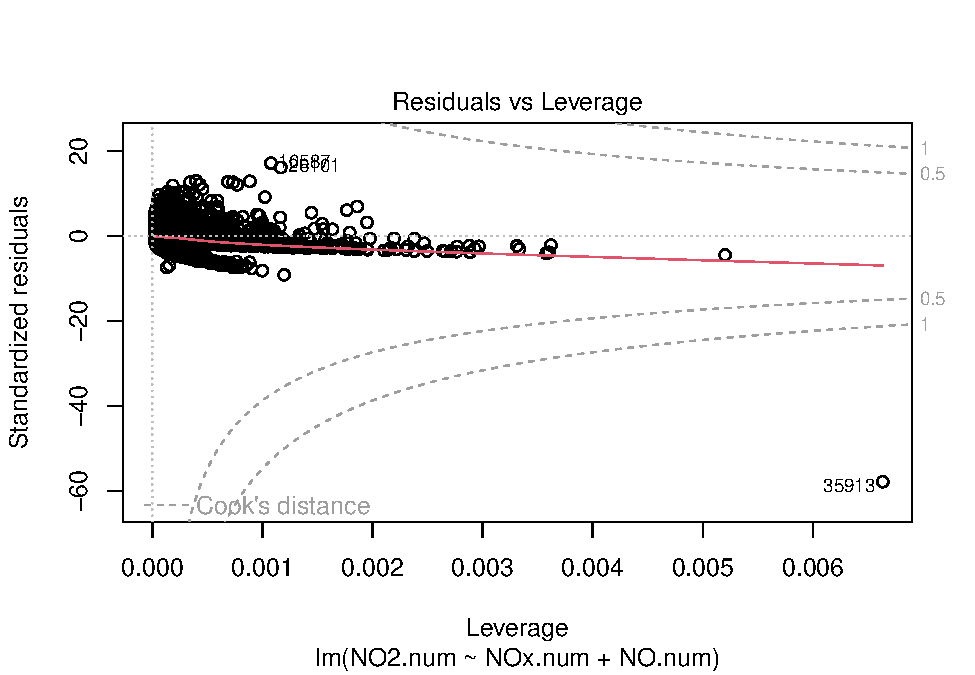
\includegraphics{ProyectoAED2023_files/figure-latex/unnamed-chunk-14-4.pdf}

El problema es que la mayoría de estaciones que no obtienen los datos de
NO2 tampoco los obtiene de la familia de los Óxidos Nitrosos.

Es por ello que se decide imputar por proximidad geográfica y en el
tiempo los datos de los Óxidos Nitrosos para posteriormente usarlo para
inferir los datos del NO2 con el modelo entrenado.

Para finalizar se imputan el resto de datos faltantes por proximidad
geográfica y temporal y se eliminan las variables que no necesitamos
para el cálculo del ICA.

Una vez tenemos imputados los datos vamos a agregar columnas adicionales
que representan de forma categórica el nivel de cada elemento desde
``Buena'' hasta ``Extremadamente desfavorable''. Para ello se ha
utilizado como guía la tabla del codebook que venía con los datos.

El código empleado se ha repetido para cada variable, ya que cada una
tiene un intervalo distnto. El código es el siguiente, que en este caso
representa el paso a categórica del SO2 en función de los intervalos:

\begin{Shaded}
\begin{Highlighting}[]
\FunctionTok{library}\NormalTok{(readr)}
\NormalTok{path }\OtherTok{\textless{}{-}}\NormalTok{ (}\StringTok{"../data/imputed\_datas.csv"}\NormalTok{)}
\NormalTok{df }\OtherTok{\textless{}{-}} \FunctionTok{read\_csv}\NormalTok{(path)}
\end{Highlighting}
\end{Shaded}

\begin{verbatim}
## New names:
## * `` -> `...1`
\end{verbatim}

\begin{verbatim}
## Warning: One or more parsing issues, call `problems()` on your data frame for details,
## e.g.:
##   dat <- vroom(...)
##   problems(dat)
\end{verbatim}

\begin{verbatim}
## Rows: 98422 Columns: 15
## -- Column specification --------------------------------------------------------
## Delimiter: ","
## chr   (4): N_PROVINCIA, N_MUNICIPIO, TIPO_AREA, geometry
## dbl  (10): ...1, ESTACION, NO2.num, O3.num, PM10.num, PM25.num, SO2.num, Dia...
## date  (1): Fecha
## 
## i Use `spec()` to retrieve the full column specification for this data.
## i Specify the column types or set `show_col_types = FALSE` to quiet this message.
\end{verbatim}

\begin{Shaded}
\begin{Highlighting}[]
\FunctionTok{list.files}\NormalTok{()}
\end{Highlighting}
\end{Shaded}

\begin{verbatim}
## [1] "appendix.tex"          "Definitions"           "mybibfile.bib"        
## [4] "ProyectoAED2023.log"   "ProyectoAED2023.pdf"   "ProyectoAED2023.Rmd"  
## [7] "ProyectoAED2023.tex"   "ProyectoAED2023_files"
\end{verbatim}

\begin{Shaded}
\begin{Highlighting}[]
\NormalTok{x }\OtherTok{\textless{}{-}}\NormalTok{ df}\SpecialCharTok{$}\NormalTok{SO2.num}
\NormalTok{y }\OtherTok{\textless{}{-}} \FunctionTok{character}\NormalTok{(}\AttributeTok{length =} \FunctionTok{length}\NormalTok{(x))}

\ControlFlowTok{for}\NormalTok{ (i }\ControlFlowTok{in} \DecValTok{1}\SpecialCharTok{:}\FunctionTok{length}\NormalTok{(x)) \{}
  \ControlFlowTok{if}\NormalTok{ (x[i] }\SpecialCharTok{\textgreater{}=} \DecValTok{0} \SpecialCharTok{\&}\NormalTok{ x[i] }\SpecialCharTok{\textless{}=} \DecValTok{100}\NormalTok{) \{}
\NormalTok{    y[i] }\OtherTok{\textless{}{-}} \StringTok{"Buena"}
\NormalTok{  \} }\ControlFlowTok{else} \ControlFlowTok{if}\NormalTok{ (x[i] }\SpecialCharTok{\textgreater{}=} \DecValTok{101} \SpecialCharTok{\&}\NormalTok{ x[i] }\SpecialCharTok{\textless{}=} \DecValTok{200}\NormalTok{) \{}
\NormalTok{    y[i] }\OtherTok{\textless{}{-}} \StringTok{"Razonablemente Buena"}
\NormalTok{  \} }\ControlFlowTok{else} \ControlFlowTok{if}\NormalTok{ (x[i] }\SpecialCharTok{\textgreater{}=} \DecValTok{201} \SpecialCharTok{\&}\NormalTok{ x[i] }\SpecialCharTok{\textless{}=} \DecValTok{350}\NormalTok{) \{}
\NormalTok{    y[i] }\OtherTok{\textless{}{-}} \StringTok{"Regular"}
\NormalTok{  \} }\ControlFlowTok{else} \ControlFlowTok{if}\NormalTok{ (x[i] }\SpecialCharTok{\textgreater{}=} \DecValTok{351} \SpecialCharTok{\&}\NormalTok{ x[i] }\SpecialCharTok{\textless{}=} \DecValTok{500}\NormalTok{) \{}
\NormalTok{    y[i] }\OtherTok{\textless{}{-}} \StringTok{"Desfavorable"}
\NormalTok{  \} }\ControlFlowTok{else} \ControlFlowTok{if}\NormalTok{ (x[i] }\SpecialCharTok{\textgreater{}=} \DecValTok{501} \SpecialCharTok{\&}\NormalTok{ x[i] }\SpecialCharTok{\textless{}=} \DecValTok{750}\NormalTok{) \{}
\NormalTok{    y[i] }\OtherTok{\textless{}{-}} \StringTok{"Muy desfavorable"}
\NormalTok{  \} }\ControlFlowTok{else} \ControlFlowTok{if}\NormalTok{ (x[i] }\SpecialCharTok{\textgreater{}=} \DecValTok{751} \SpecialCharTok{\&}\NormalTok{ x[i] }\SpecialCharTok{\textless{}=} \DecValTok{1250}\NormalTok{) \{}
\NormalTok{    y[i] }\OtherTok{\textless{}{-}} \StringTok{"Extremadamente desfavorable"}
\NormalTok{  \}}
\NormalTok{\}}

\NormalTok{df}\SpecialCharTok{$}\NormalTok{SO2.cat }\OtherTok{\textless{}{-}}\NormalTok{ y}
\end{Highlighting}
\end{Shaded}

Una vez se obtiene el valor categórico de cada variable, se establece el
Indice global diario como el peor de los individuales.

\begin{Shaded}
\begin{Highlighting}[]
\NormalTok{df }\OtherTok{\textless{}{-}} \FunctionTok{read\_csv}\NormalTok{(}\StringTok{"../data/dataset\_final.csv"}\NormalTok{, }
    \AttributeTok{col\_types =} \FunctionTok{cols}\NormalTok{(}\AttributeTok{...1 =} \FunctionTok{col\_skip}\NormalTok{(), }\AttributeTok{...2 =} \FunctionTok{col\_skip}\NormalTok{(), }
        \AttributeTok{Fecha =} \FunctionTok{col\_date}\NormalTok{(}\AttributeTok{format =} \StringTok{"\%Y{-}\%m{-}\%d"}\NormalTok{)))}
\NormalTok{levels}\OtherTok{\textless{}{-}}\FunctionTok{c}\NormalTok{(}\StringTok{\textquotesingle{}Buena\textquotesingle{}}\NormalTok{,}\StringTok{\textquotesingle{}Razonablemente Buena\textquotesingle{}}\NormalTok{,}\StringTok{\textquotesingle{}Regular\textquotesingle{}}\NormalTok{,}\StringTok{\textquotesingle{}Desfavorable\textquotesingle{}}\NormalTok{,}\StringTok{\textquotesingle{}Muy desfavorable\textquotesingle{}}\NormalTok{,}\StringTok{\textquotesingle{}Extremadamente desfavorable\textquotesingle{}}\NormalTok{)}
\NormalTok{df}\OtherTok{\textless{}{-}}\NormalTok{df}\SpecialCharTok{\%\textgreater{}\%} \FunctionTok{mutate}\NormalTok{(}\AttributeTok{TIPO\_AREA=}\FunctionTok{as.factor}\NormalTok{(TIPO\_AREA))}\SpecialCharTok{\%\textgreater{}\%}\FunctionTok{mutate}\NormalTok{(}\FunctionTok{across}\NormalTok{(}\FunctionTok{c}\NormalTok{(}\FunctionTok{ends\_with}\NormalTok{(}\StringTok{\textquotesingle{}.cat\textquotesingle{}}\NormalTok{)), factor,}\AttributeTok{level=}\NormalTok{levels))}\SpecialCharTok{\%\textgreater{}\%} \FunctionTok{mutate}\NormalTok{(}\AttributeTok{ICA=}\FunctionTok{factor}\NormalTok{(ICA,}\AttributeTok{level=}\NormalTok{levels))}
\FunctionTok{kable}\NormalTok{(}\FunctionTok{head}\NormalTok{(df))}
\end{Highlighting}
\end{Shaded}

\begin{tabular}{l|l|l|l|r|r|r|r|r|r|r|r|r|l|l|l|l|l|l|l}
\hline
N\_PROVINCIA & N\_MUNICIPIO & TIPO\_AREA & Fecha & ESTACION & NO2.num & O3.num & PM10.num & PM25.num & SO2.num & Dias & X\_UTM30N & Y\_UTM30N & geometry & NO2.cat & O3.cat & PM10.cat & PM25.cat & SO2.cat & ICA\\
\hline
CASTELLÓN/CASTELLÓ & TORRE ENDOMÉNECH & RURAL & 2018-07-29 & 1 & 7 & 98 & 28 & 24 & 4 & 209 & 748380.2 & 4461758 & c(748380.171727976, 4461757.68088724) & Buena & Razonablemente Buena & Razonablemente Buena & Regular & Buena & Regular\\
\hline
CASTELLÓN/CASTELLÓ & TORRE ENDOMÉNECH & RURAL & 2018-02-15 & 1 & 30 & 68 & 16 & 10 & 3 & 45 & 748380.2 & 4461758 & c(748380.171727976, 4461757.68088724) & Buena & Razonablemente Buena & Buena & Buena & Buena & Razonablemente Buena\\
\hline
CASTELLÓN/CASTELLÓ & TORRE ENDOMÉNECH & RURAL & 2018-11-14 & 1 & 38 & 89 & 22 & 15 & 3 & 317 & 748380.2 & 4461758 & c(748380.171727976, 4461757.68088724) & Buena & Razonablemente Buena & Razonablemente Buena & Razonablemente Buena & Buena & Razonablemente Buena\\
\hline
CASTELLÓN/CASTELLÓ & TORRE ENDOMÉNECH & RURAL & 2018-08-02 & 1 & 7 & 99 & 49 & 44 & 4 & 213 & 748380.2 & 4461758 & c(748380.171727976, 4461757.68088724) & Buena & Razonablemente Buena & Regular & Desfavorable & Buena & Desfavorable\\
\hline
CASTELLÓN/CASTELLÓ & TORRE ENDOMÉNECH & RURAL & 2018-11-24 & 1 & 38 & 84 & 4 & 3 & 3 & 327 & 748380.2 & 4461758 & c(748380.171727976, 4461757.68088724) & Buena & Razonablemente Buena & Buena & Buena & Buena & Razonablemente Buena\\
\hline
CASTELLÓN/CASTELLÓ & TORRE ENDOMÉNECH & RURAL & 2018-08-27 & 1 & 13 & 84 & 22 & 14 & 4 & 238 & 748380.2 & 4461758 & c(748380.171727976, 4461757.68088724) & Buena & Razonablemente Buena & Razonablemente Buena & Razonablemente Buena & Buena & Razonablemente Buena\\
\hline
\end{tabular}

\hypertarget{anuxe1lisis-univariante}{%
\section{Análisis Univariante}\label{anuxe1lisis-univariante}}

En esta sección, procederemos a llevar a cabo un análisis univariante
sobre el conjunto de datos previamente procesado. El propósito principal
de esta evaluación consiste en examinar individualmente cada variable
presente en el dataset, con el objetivo de obtener un panorama detallado
de su distribución y variabilidad.

En primer lugar, para tener una visión global de este dataset sacamos un
resumen estadístico

\begin{verbatim}
##  N_PROVINCIA        N_MUNICIPIO            TIPO_AREA         Fecha           
##  Length:98422       Length:98422       RURAL    :23413   Min.   :2018-01-01  
##  Class :character   Class :character   SUBURBANA:44449   1st Qu.:2019-04-07  
##  Mode  :character   Mode  :character   URBANA   :30560   Median :2020-07-06  
##                                                          Mean   :2020-07-04  
##                                                          3rd Qu.:2021-10-04  
##                                                          Max.   :2022-12-31  
##     ESTACION         NO2.num           O3.num         PM10.num     
##  Min.   : 1.000   Min.   :  1.00   Min.   :  1.0   Min.   :  1.00  
##  1st Qu.: 1.000   1st Qu.:  9.00   1st Qu.: 74.0   1st Qu.: 12.00  
##  Median : 3.000   Median : 21.00   Median : 88.0   Median : 22.00  
##  Mean   : 9.192   Mean   : 27.91   Mean   : 88.6   Mean   : 29.34  
##  3rd Qu.: 8.000   3rd Qu.: 41.00   3rd Qu.:103.0   3rd Qu.: 37.00  
##  Max.   :54.000   Max.   :229.00   Max.   :207.0   Max.   :757.00  
##     PM25.num         SO2.num             Dias         X_UTM30N     
##  Min.   :  0.00   Min.   :  1.000   Min.   :   0   Min.   :647644  
##  1st Qu.:  7.00   1st Qu.:  3.000   1st Qu.: 461   1st Qu.:715944  
##  Median : 12.00   Median :  4.000   Median : 917   Median :725781  
##  Mean   : 15.42   Mean   :  6.359   Mean   : 916   Mean   :723388  
##  3rd Qu.: 19.00   3rd Qu.:  6.000   3rd Qu.:1372   3rd Qu.:739720  
##  Max.   :296.00   Max.   :239.000   Max.   :1825   Max.   :785582  
##     Y_UTM30N         geometry                                NO2.cat     
##  Min.   :4207346   Length:98422       Buena                      :73677  
##  1st Qu.:4316834   Class :character   Razonablemente Buena       :22851  
##  Median :4380180   Mode  :character   Regular                    : 1678  
##  Mean   :4372626                      Desfavorable               :  216  
##  3rd Qu.:4427433                      Muy desfavorable           :    0  
##  Max.   :4513195                      Extremadamente desfavorable:    0  
##                          O3.cat                             PM10.cat    
##  Buena                      : 3477   Buena                      :45050  
##  Razonablemente Buena       :66563   Razonablemente Buena       :32606  
##  Regular                    :25929   Regular                    : 7181  
##  Desfavorable               : 2453   Desfavorable               :11447  
##  Muy desfavorable           :    0   Muy desfavorable           : 1478  
##  Extremadamente desfavorable:    0   Extremadamente desfavorable:  660  
##                         PM25.cat                            SO2.cat     
##  Buena                      :44243   Buena                      :98334  
##  Razonablemente Buena       :31682   Razonablemente Buena       :   86  
##  Regular                    : 7987   Regular                    :    2  
##  Desfavorable               :11839   Desfavorable               :    0  
##  Muy desfavorable           : 1686   Muy desfavorable           :    0  
##  Extremadamente desfavorable:  985   Extremadamente desfavorable:    0  
##                           ICA       
##  Buena                      :  552  
##  Razonablemente Buena       :46805  
##  Regular                    :27844  
##  Desfavorable               :18838  
##  Muy desfavorable           : 2841  
##  Extremadamente desfavorable: 1542
\end{verbatim}

Una vez obtenidos los estadísticos. Visualizamos nuestras variables.

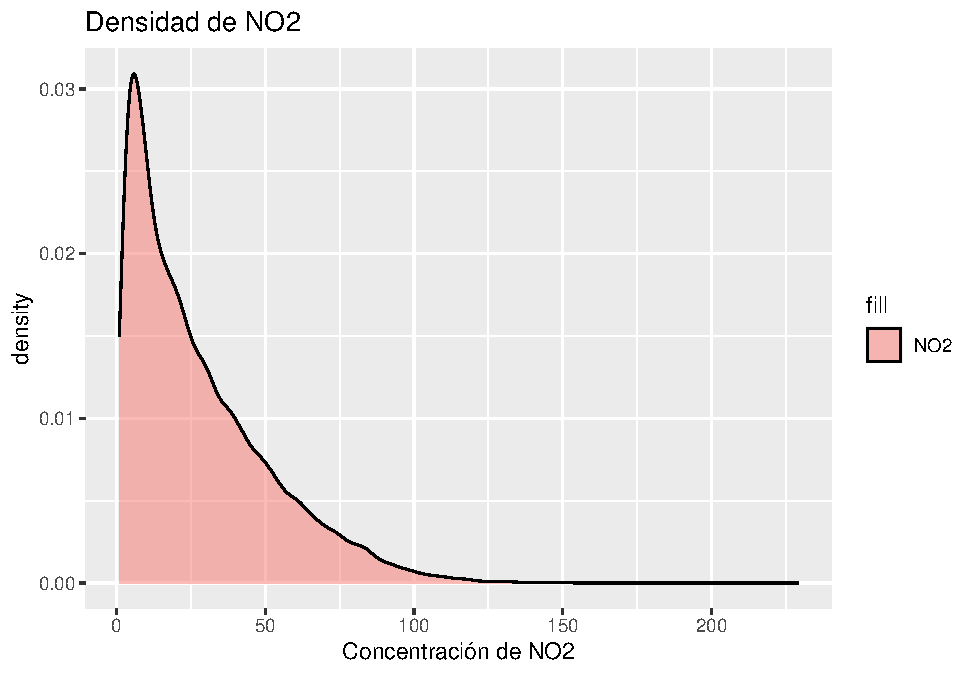
\includegraphics{ProyectoAED2023_files/figure-latex/unnamed-chunk-21-1.pdf}

La representación gráfica previa proporciona una visión general de la
concentración de cada elemento en nuestro conjunto de datos. La
representación más notable en términos de su estructura y forma
corresponde al elemento \(O_{3}\), ya que parece seguir una distribución
gaussiana. Los datos están distribuidos de manera uniforme a lo largo
del eje x, que representa la concentración, y muestran una distribución
alrededor de la media y la mediana, ambas con valores muy similares,
como se confirmó en los estadísticos previamente descritos. (88.60 y
88.00 respectivamente).

En contraste, las representaciones de los otros elementos exhiben una
asimetría significativa, con valores relativamente altos al principio
seguidos de una disminución. Estas observaciones son respaldadas
numéricamente por los estadísticos calculados anteriormente. Por
ejemplo, al considerar el elemento \(S0_{2}\), se observa un valor
máximo de 239,000. Sin embargo, la media calculada es de 6,359, un valor
considerablemente distante del máximo mencionado. Además, el valor
mínimo es 1, mientras que la mediana es 4,000. Estas discrepancias
justifican la representación gráfica de esta información. Esto mismo
sucedería con los elementos restantes.

A continuación, procederemos a visualizar la evolución de los compuestos
químicos a lo largo del tiempo, con el objetivo de realizar un análisis
más exhaustivo sobre la calidad del aire.

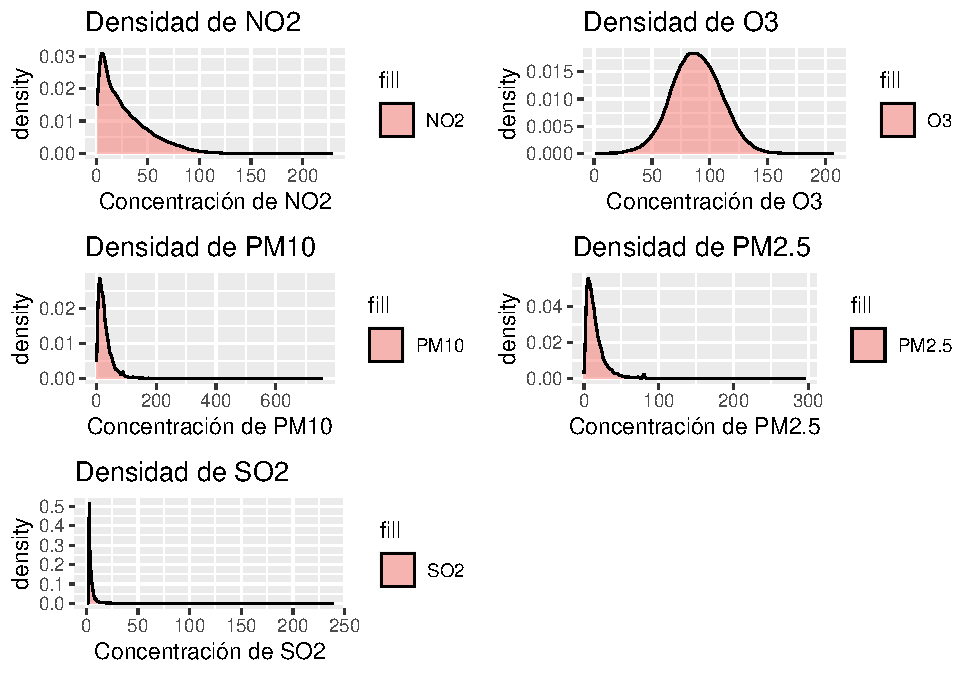
\includegraphics{ProyectoAED2023_files/figure-latex/unnamed-chunk-22-1.pdf}

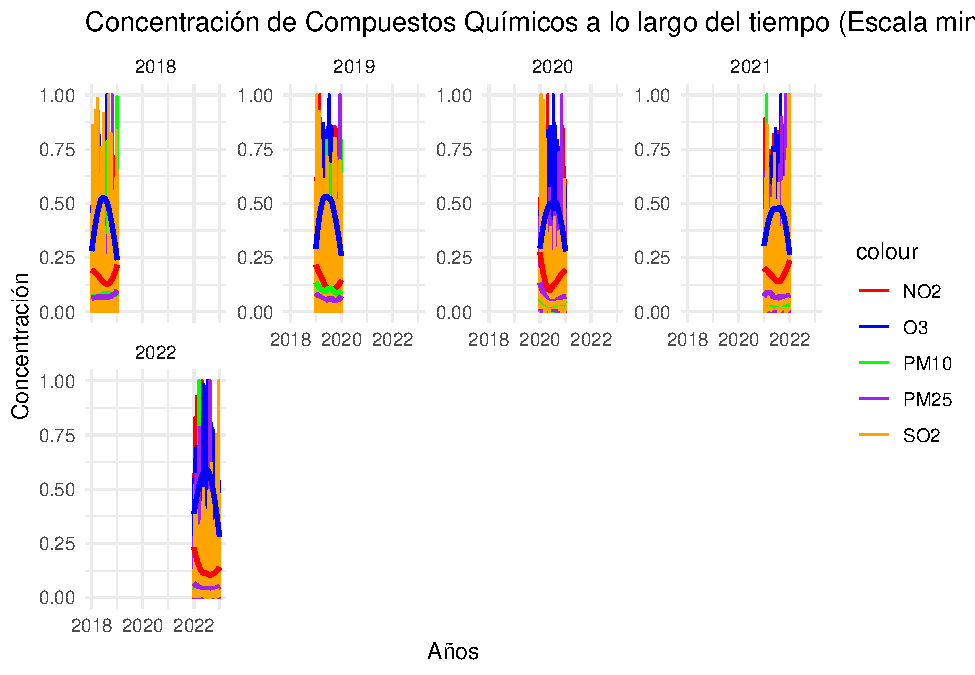
\includegraphics{ProyectoAED2023_files/figure-latex/unnamed-chunk-23-1.pdf}

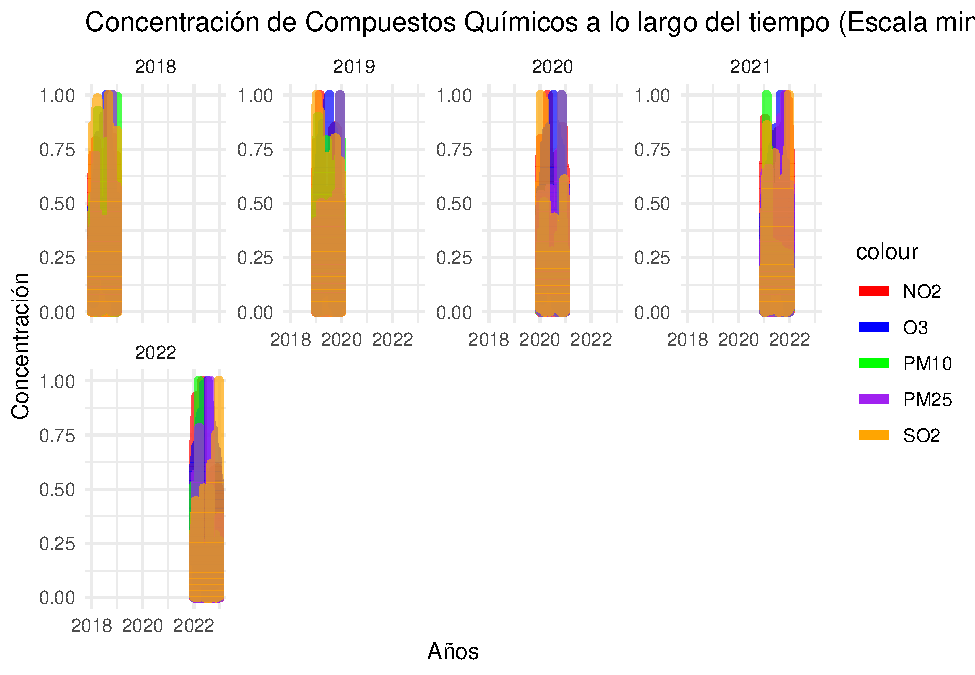
\includegraphics{ProyectoAED2023_files/figure-latex/unnamed-chunk-24-1.pdf}

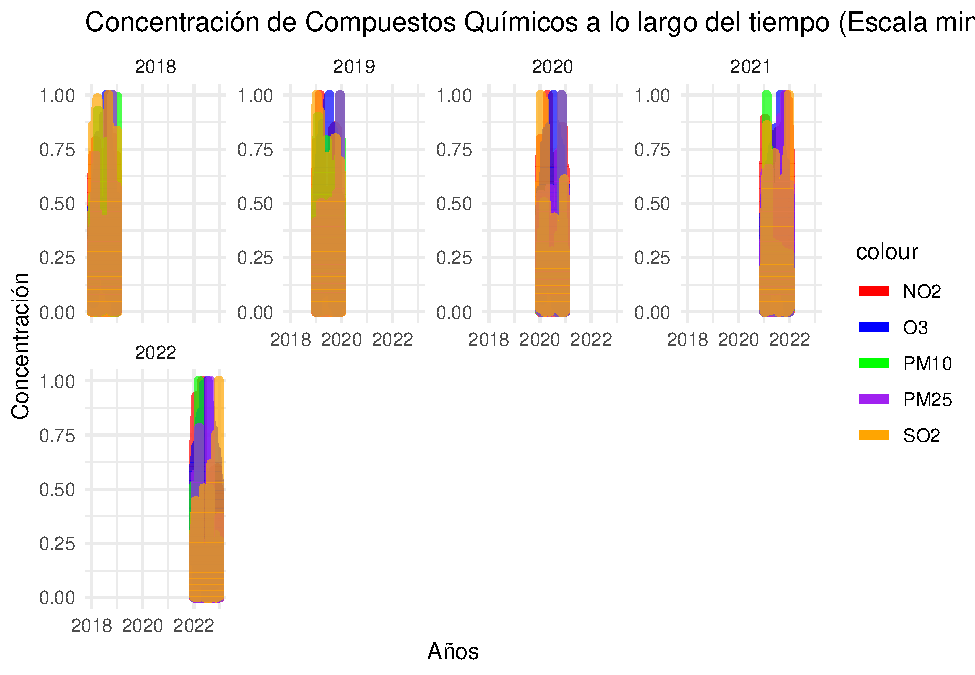
\includegraphics{ProyectoAED2023_files/figure-latex/unnamed-chunk-25-1.pdf}

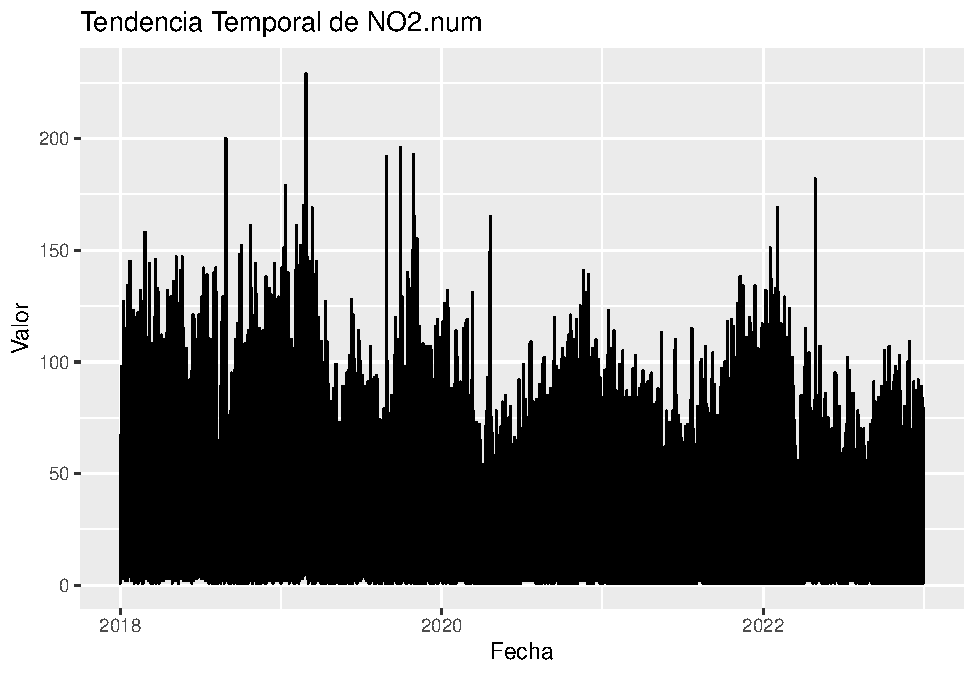
\includegraphics{ProyectoAED2023_files/figure-latex/unnamed-chunk-27-1.pdf}

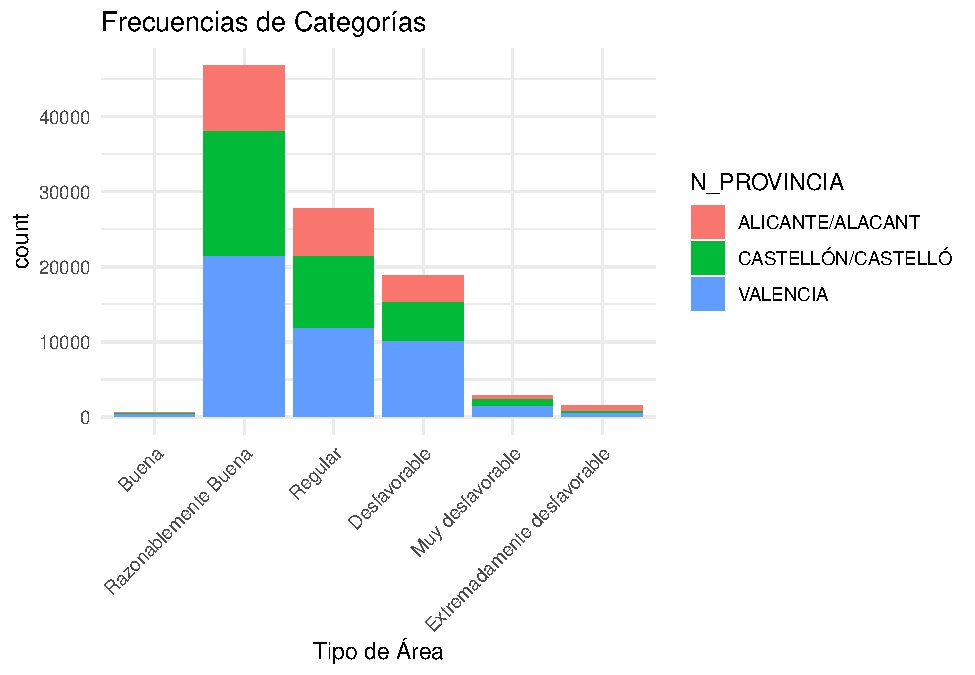
\includegraphics{ProyectoAED2023_files/figure-latex/unnamed-chunk-28-1.pdf}

Pensar que hacer con los nombres

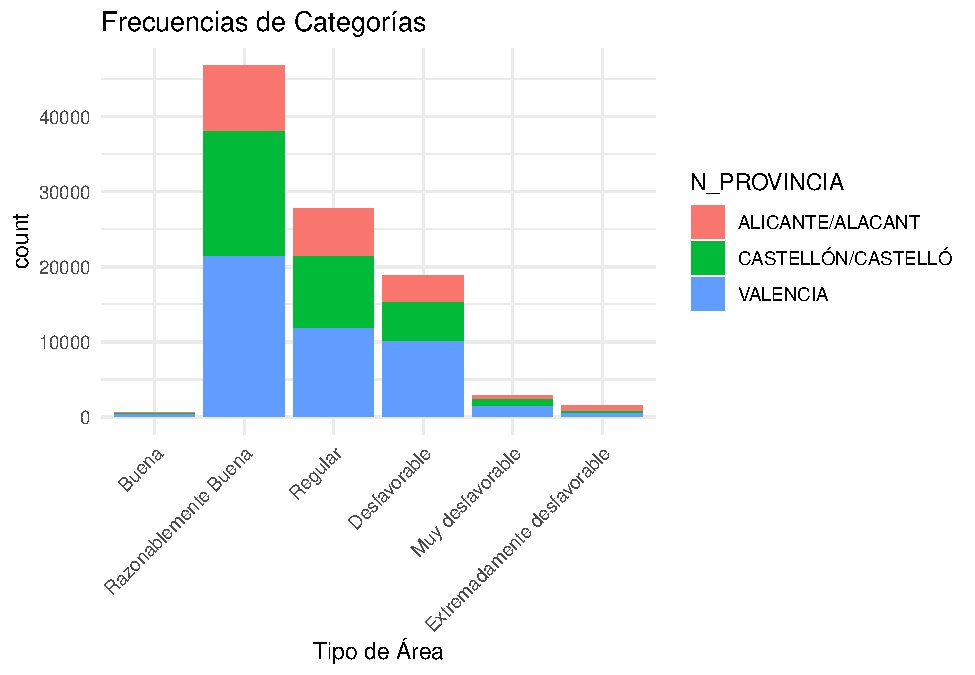
\includegraphics{ProyectoAED2023_files/figure-latex/unnamed-chunk-29-1.pdf}

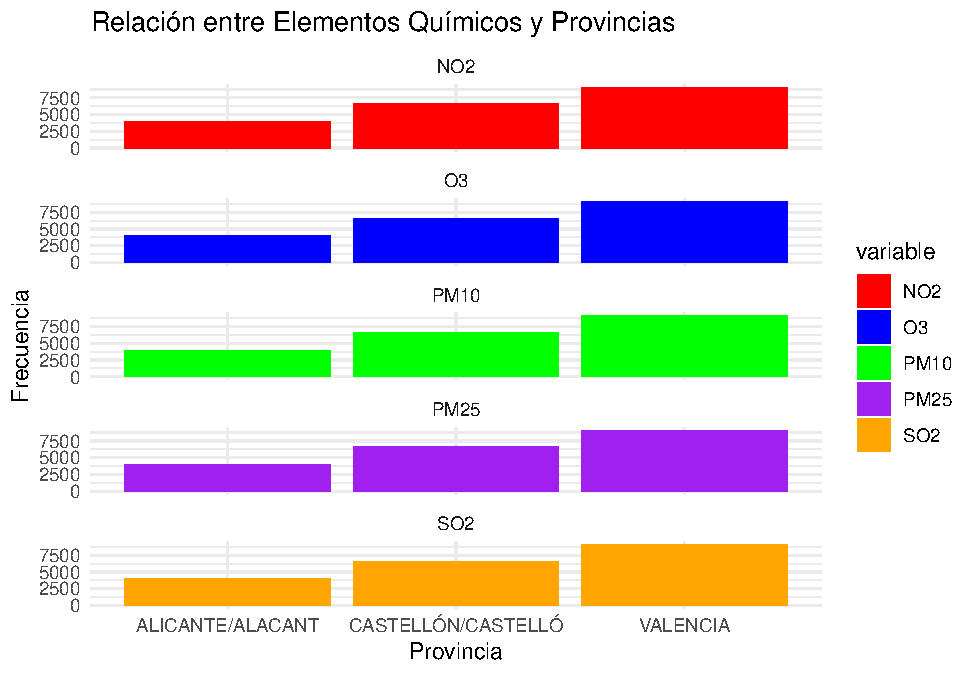
\includegraphics{ProyectoAED2023_files/figure-latex/unnamed-chunk-30-1.pdf}

\hypertarget{anuxe1lisis-bivariante}{%
\section{Análisis Bivariante}\label{anuxe1lisis-bivariante}}

Para realizar el análisis bivariante primer observaremos como se
relacionan todas las variables entre sí

Primero vamos a realizar un \texttt{ggpairs} y un \texttt{ggcorr}para
relacionar todos los elementos químicos con todos (valores numéricos)

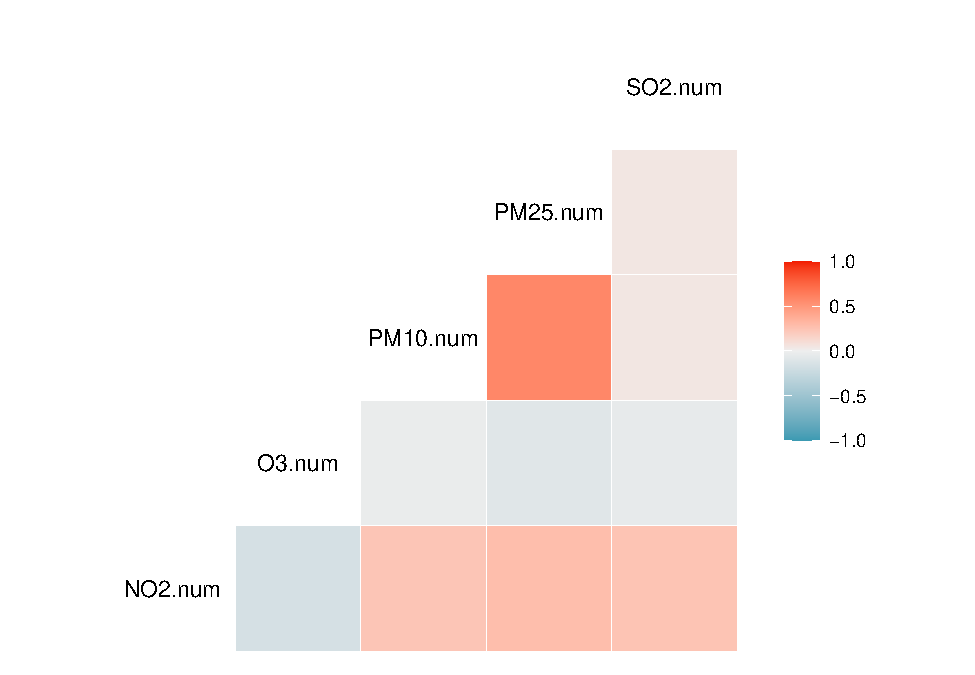
\includegraphics{ProyectoAED2023_files/figure-latex/unnamed-chunk-32-1.pdf}

\begin{center}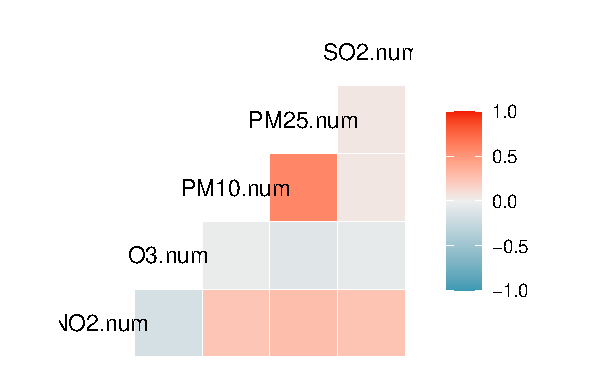
\includegraphics{ProyectoAED2023_files/figure-latex/unnamed-chunk-33-1} \end{center}

Como podemos ver, la relación de las variables no es clara. De forma
general podemos decir que las variables son bastante independientes
entre sí.Como excepción podríamos hablar de las variables PM10 y PM25

Ahora mostraremos las matrices de covaraianza y correlación con Pearson
y Spearman

\begin{verbatim}
## [1] "Matriz de covarianza"
\end{verbatim}

\begin{verbatim}
##            NO2.num     O3.num  PM10.num   PM25.num   SO2.num
## NO2.num  558.50671 -79.413288 159.80303  91.904814 49.402858
## O3.num   -79.41329 453.671329 -16.17258 -26.902899 -8.273695
## PM10.num 159.80303 -16.172582 829.28383 232.735487 11.902949
## PM25.num  91.90481 -26.902899 232.73549 194.558055  5.841597
## SO2.num   49.40286  -8.273695  11.90295   5.841597 73.528576
\end{verbatim}

\begin{verbatim}
## [1] "Matriz de correlacion (Spearman)"
\end{verbatim}

\begin{verbatim}
##             NO2.num      O3.num   PM10.num    PM25.num     SO2.num
## NO2.num   1.0000000 -0.13546859 0.32082787  0.31022061  0.35079803
## O3.num   -0.1354686  1.00000000 0.01720491 -0.02215115 -0.03290146
## PM10.num  0.3208279  0.01720491 1.00000000  0.72516556  0.17837261
## PM25.num  0.3102206 -0.02215115 0.72516556  1.00000000  0.14920745
## SO2.num   0.3507980 -0.03290146 0.17837261  0.14920745  1.00000000
\end{verbatim}

\begin{verbatim}
## [1] "Matriz de correlacion (Pearson)"
\end{verbatim}

\begin{verbatim}
##             NO2.num      O3.num    PM10.num    PM25.num     SO2.num
## NO2.num   1.0000000 -0.15776415  0.23481143  0.27880429  0.24378658
## O3.num   -0.1577641  1.00000000 -0.02636678 -0.09055320 -0.04530027
## PM10.num  0.2348114 -0.02636678  1.00000000  0.57941055  0.04820309
## PM25.num  0.2788043 -0.09055320  0.57941055  1.00000000  0.04884036
## SO2.num   0.2437866 -0.04530027  0.04820309  0.04884036  1.00000000
\end{verbatim}

Ya que hemos visto que las variables PM10 y PM25 parece que tengan
alguna relación, vamos a relacionar sus equivalentes categóricas para
ver si la hipótesis nula de que son independientes se cumple o no.

\begin{Shaded}
\begin{Highlighting}[]
\FunctionTok{chisq.test}\NormalTok{(df}\SpecialCharTok{$}\NormalTok{PM10.cat, df}\SpecialCharTok{$}\NormalTok{PM25.cat, }\AttributeTok{correct =}\NormalTok{ F)}
\end{Highlighting}
\end{Shaded}

\begin{verbatim}
## 
##  Pearson's Chi-squared test
## 
## data:  df$PM10.cat and df$PM25.cat
## X-squared = 57030, df = 25, p-value < 2.2e-16
\end{verbatim}

Podemos ver que el p-valor es muy pequeño, luego podemos rechazar la
hipótesis de que no están relacionadas.

Este efecto es más grande en las categóricas, ya que ``medimos'' por
intervalos. Por lo que podemos decir que sí tienen alguna relación entre
ellas

\hypertarget{no2}{%
\subsection{NO2}\label{no2}}

\begin{center}\includegraphics{ProyectoAED2023_files/figure-latex/unnamed-chunk-37-1} \end{center}

\begin{verbatim}
##             NO2.num      O3.num    PM10.num    PM25.num     SO2.num
## NO2.num   1.0000000 -0.15776415  0.23481143  0.27880429  0.24378658
## O3.num   -0.1577641  1.00000000 -0.02636678 -0.09055320 -0.04530027
## PM10.num  0.2348114 -0.02636678  1.00000000  0.57941055  0.04820309
## PM25.num  0.2788043 -0.09055320  0.57941055  1.00000000  0.04884036
## SO2.num   0.2437866 -0.04530027  0.04820309  0.04884036  1.00000000
\end{verbatim}

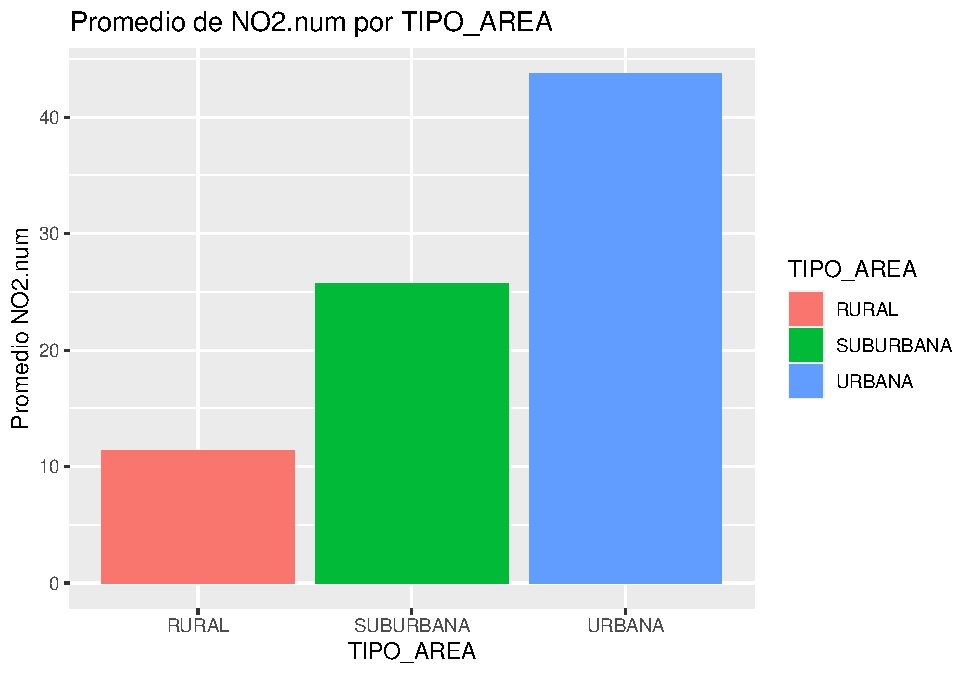
\includegraphics{ProyectoAED2023_files/figure-latex/unnamed-chunk-39-1.pdf}

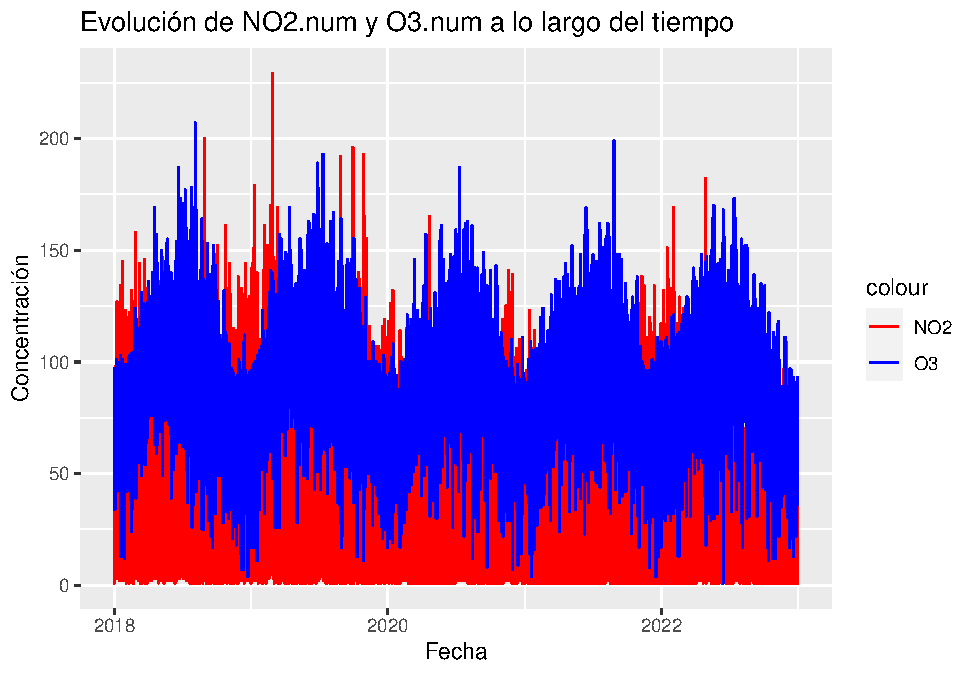
\includegraphics{ProyectoAED2023_files/figure-latex/unnamed-chunk-40-1.pdf}

\includegraphics{ProyectoAED2023_files/figure-latex/unnamed-chunk-41-1.pdf}

Vamos a mostrar ahora un histograma de la cantidad de días en los cuales
ha habido cada uno de los diferentes índices de la calidad del aire.
Para calcular esto debemos coger todas las mediciones de un mismo día y
quedarnos con la peor, y esta es la calidad de aire para ese día.

\begin{center}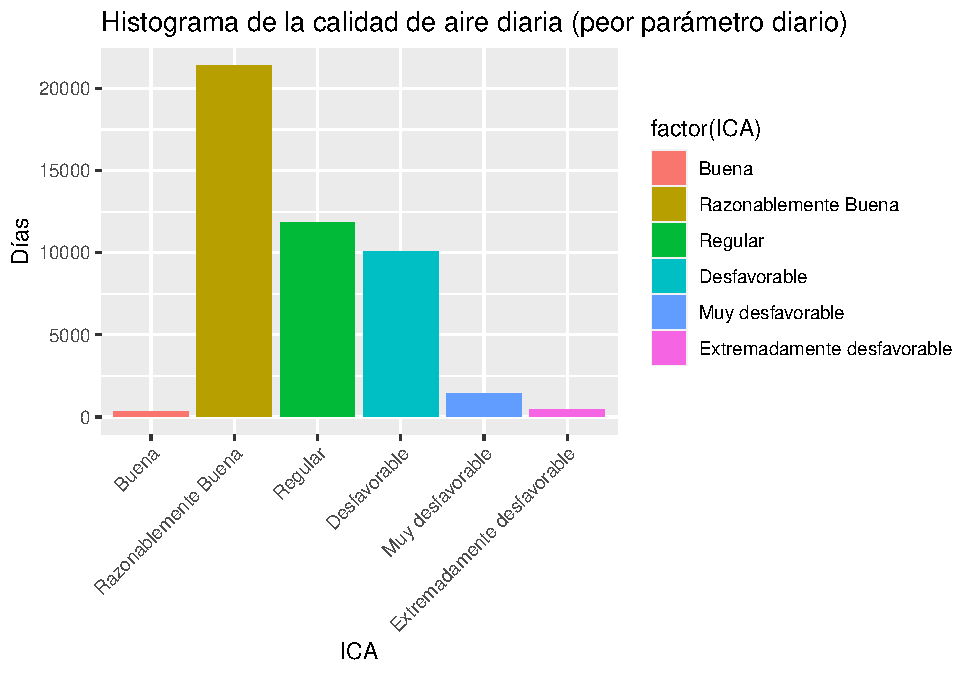
\includegraphics{ProyectoAED2023_files/figure-latex/unnamed-chunk-44-1} \end{center}

Vamos ahora a probar, por ejemplo, a sacar la misma gráfica usando solo
los datos de la provincia de València

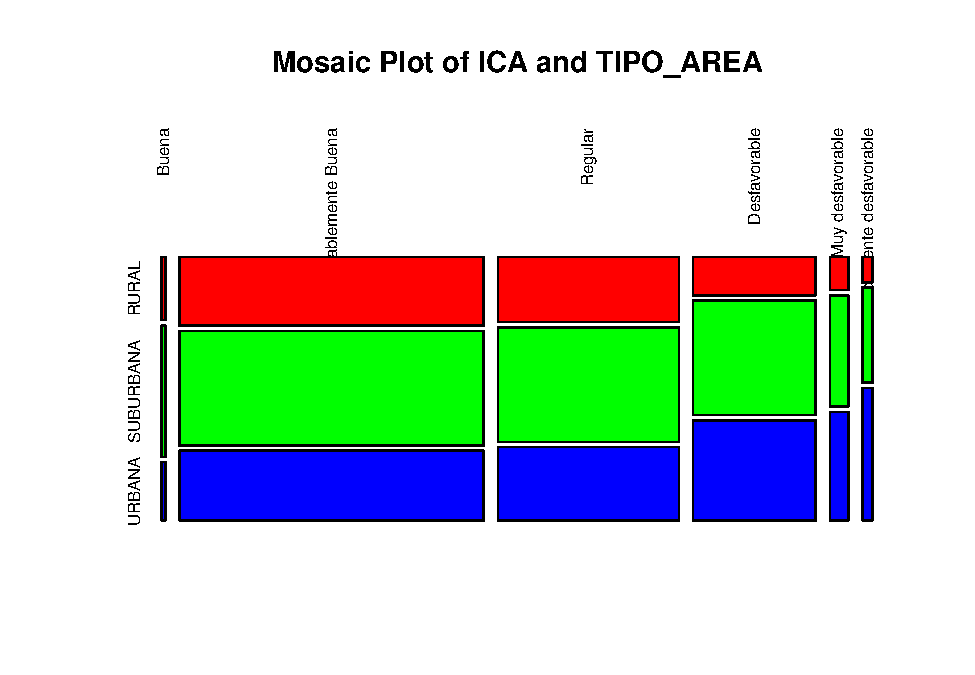
\includegraphics{ProyectoAED2023_files/figure-latex/unnamed-chunk-45-1.pdf}

Podemos observar que la distribución de los datos parece mantenerse en
ambos casos. Hay pocos días donde la calidad del aire sea buena. Por
otro lado el parámetro más frecuente es el de razonablemente buena, a
partir del cual los sucesivos van bajando hasta llegar a extremadamente
desfavorable.

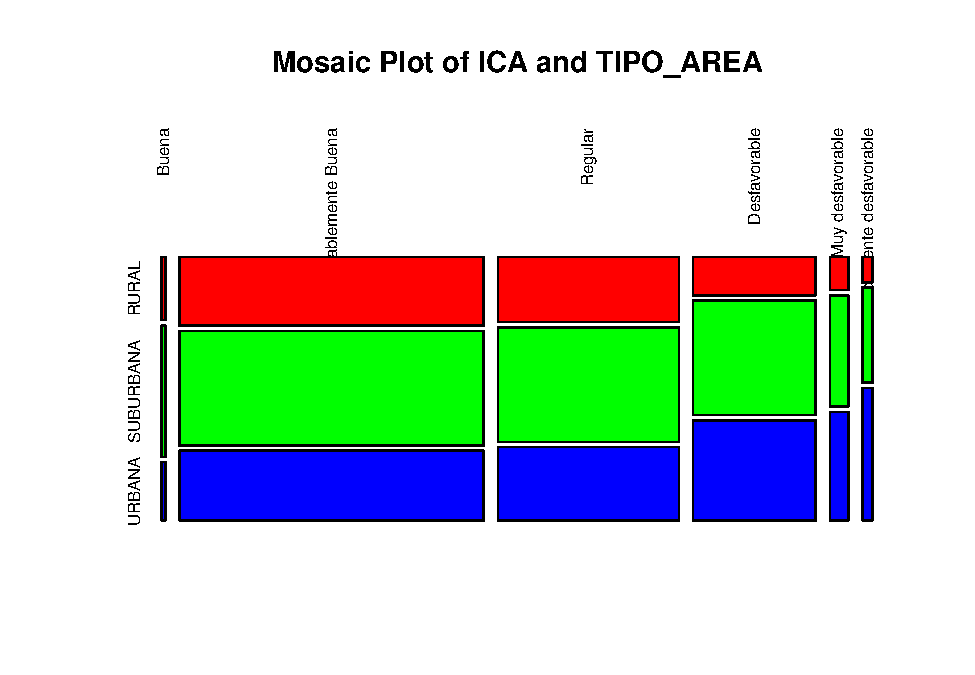
\includegraphics{ProyectoAED2023_files/figure-latex/unnamed-chunk-46-1.pdf}
Con el mosaic plot podemos observar como a pesar de que la cantidad de
días que el aire tiene una calidad buena no es muy diferente entre las
zonas, en las zonas rurales hay menos días con calidades peores.

\begin{Shaded}
\begin{Highlighting}[]
\CommentTok{\# \# Instalar y cargar las librerías}
\CommentTok{\# library(sf)}
\CommentTok{\# library(leaflet)}
\CommentTok{\# }
\CommentTok{\# \# Cargar datos desde el archivo JSON}
\CommentTok{\# ruta\_al\_archivo \textless{}{-} "../data/CV{-}MAP.json"}
\CommentTok{\# datos\_sf \textless{}{-} st\_read(ruta\_al\_archivo)}
\CommentTok{\# }
\CommentTok{\# \# Crear un mapa interactivo con Leaflet}
\CommentTok{\# mapa \textless{}{-} leaflet() \%\textgreater{}\%}
\CommentTok{\#   addTiles() \%\textgreater{}\%}
\CommentTok{\#   addMarkers(data = datos\_sf, \textasciitilde{}X\_UTM30N, \textasciitilde{}Y\_UTM30N, popup = \textasciitilde{}as.character(geometry))}
\CommentTok{\# }
\CommentTok{\# \# Mostrar el mapa}
\CommentTok{\# mapa}
\end{Highlighting}
\end{Shaded}

\hypertarget{conclusiones}{%
\section{Conclusiones}\label{conclusiones}}

\hypertarget{results}{%
\section{Results}\label{results}}

This section may be divided by subheadings. It should provide a concise
and precise description of the experimental results, their
interpretation as well as the experimental conclusions that can be
drawn.

\hypertarget{subsection-heading-here}{%
\subsection{Subsection Heading Here}\label{subsection-heading-here}}

Subsection text here.

\hypertarget{subsubsection-heading-here}{%
\subsubsection{Subsubsection Heading
Here}\label{subsubsection-heading-here}}

Bulleted lists look like this:

\begin{itemize}
\tightlist
\item
  First bullet
\item
  Second bullet
\item
  Third bullet
\end{itemize}

Numbered lists can be added as follows:

\begin{enumerate}
\def\labelenumi{\arabic{enumi}.}
\tightlist
\item
  First item
\item
  Second item
\item
  Third item
\end{enumerate}

The text continues here.

\hypertarget{figures-tables-and-schemes}{%
\subsection{Figures, Tables and
Schemes}\label{figures-tables-and-schemes}}

All figures and tables should be cited in the main text as Figure
\ref{fig:fig1}, \ref{tab:tab1}, etc. To get cross-reference to figure
generated by R chunks include the
\texttt{\textbackslash{}\textbackslash{}label\{\}} tag in the
\texttt{fig.cap} attribute of the R chunk:
\texttt{fig.cap\ =\ "Fancy\ Caption\textbackslash{}\textbackslash{}label\{fig:plot\}"}.

\begin{figure}
\centering
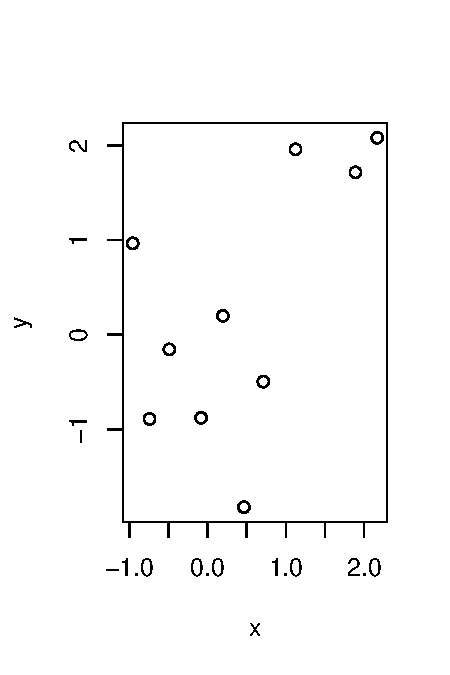
\includegraphics{ProyectoAED2023_files/figure-latex/fig1-1.pdf}
\caption{A figure added with a code chunk.\label{fig:fig1}}
\end{figure}

When making tables using \texttt{kable}, it is suggested to use the
\texttt{format="latex"} and \texttt{tabl.envir="table"} arguments to
ensure table numbering and compatibility with the mdpi document class.

\begin{table}[H]

\caption{\label{tab:tab1}This is a table caption. Tables should be placed in the 
             main text near to the first time they are~cited.}
\begin{tabular}[t]{lccc}
\toprule
  & mpg & cyl & disp\\
\midrule
Mazda RX4 & 21.0 & 6 & 160\\
Mazda RX4 Wag & 21.0 & 6 & 160\\
Datsun 710 & 22.8 & 4 & 108\\
Hornet 4 Drive & 21.4 & 6 & 258\\
Hornet Sportabout & 18.7 & 8 & 360\\
\bottomrule
\end{tabular}
\end{table}

For a very wide table, landscape layouts are allowed.

\startlandscape

\begin{table}[H]

\caption{\label{tab:tab2}This is a very wide table}
\begin{tabular}[t]{cccc}
\toprule
Title.1 & Title.2 & Title.3 & Title.4\\
\midrule
Entry 1 & Data & Data & This cell has some longer content that runs over
                               two lines\\
Entry 2 & Data & Data & Data\\
\bottomrule
\end{tabular}
\end{table}

\finishlandscape

\hypertarget{formatting-of-mathematical-components}{%
\subsection{Formatting of Mathematical
Components}\label{formatting-of-mathematical-components}}

This is an example of an equation:

\[
a = 1.
\]

If you want numbered equations use Latex and wrap in the equation
environment:

\begin{equation}
a = 1,
\end{equation}

the text following an equation need not be a new paragraph. Please
punctuate equations as regular text.

This is the example 2 of equation:

\begin{adjustwidth}{-\extralength}{0cm}
\begin{equation}
a = b + c + d + e + f + g + h + i + j + k + l + m + n + o + p + q + r + s + t + 
u + v + w + x + y + z
\end{equation}
\end{adjustwidth}

Theorem-type environments (including propositions, lemmas, corollaries
etc.) can be formatted as follows:

Example of a theorem:

\begin{Theorem}
Example text of a theorem

\end{Theorem}

The text continues here. Proofs must be formatted as follows:

Example of a proof:

\begin{proof}[Proof of Theorem1]
Text of the proof. Note that the phrase ``of Theorem 1'\,' is optional
if it is clear which theorem is being referred to.

\end{proof}

The text continues here.

\hypertarget{discussion}{%
\section{Discussion}\label{discussion}}

Authors should discuss the results and how they can be interpreted in
perspective of previous studies and of the working hypotheses. The
findings and their implications should be discussed in the broadest
context possible. Future research directions may also be highlighted.

\hypertarget{conclusion}{%
\section{Conclusion}\label{conclusion}}

This section is not mandatory, but can be added to the manuscript if the
discussion is unusually long or complex.

\hypertarget{patents}{%
\section{Patents}\label{patents}}

This section is not mandatory, but may be added if there are patents
resulting from the work reported in this manuscript.

%%%%%%%%%%%%%%%%%%%%%%%%%%%%%%%%%%%%%%%%%%

\vspace{6pt}

%%%%%%%%%%%%%%%%%%%%%%%%%%%%%%%%%%%%%%%%%%
%% optional
\supplementary{The following supporting information can be downloaded
at:\\
\linksupplementary{s1}, Figure S1: title; Table S1: title; Video S1:
title.}

% Only for the journal Methods and Protocols:
% If you wish to submit a video article, please do so with any other supplementary material.
% \supplementary{The following supporting information can be downloaded at: \linksupplementary{s1}, Figure S1: title; Table S1: title; Video S1: title. A supporting video article is available at doi: link.}

%%%%%%%%%%%%%%%%%%%%%%%%%%%%%%%%%%%%%%%%%%
\authorcontributions{For research articles with several authors, a short
paragraph specifying their individual contributions must be provided.
The following statements should be used ``X.X. and Y.Y. conceive and
designed the experiments; X.X. performed the experiments; X.X. and Y.Y.
analyzed the data; W.W. contributed reagents/materials/analysis tools;
Y.Y. wrote the paper.'\,' Authorship must be limited to those who have
contributed substantially to the work reported.}

\funding{Please add:
\texttt{This\ research\ received\ no\ external\ funding\textquotesingle{}\textquotesingle{}\ or}This
research was funded by NAME OF FUNDER grant number XXX.'\,' and and
``The APC was funded by XXX'\,'. Check carefully that the details given
are accurate and use the standard spelling of funding agency names at
\url{https://search.crossref.org/funding}, any errors may affect your
future funding.}

\institutionalreview{In this section, you should add the Institutional
Review Board Statement and approval number, if relevant to your study.
You might choose to exclude this statement if the study did not require
ethical approval. Please note that the Editorial Office might ask you
for further information. Please add ``The study was conducted in
accordance with the Declaration of Helsinki, and approved by the
Institutional Review Board (or Ethics Committee) of NAME OF INSTITUTE
(protocol code XXX and date of approval).'' for studies involving
humans. OR ``The animal study protocol was approved by the Institutional
Review Board (or Ethics Committee) of NAME OF INSTITUTE (protocol code
XXX and date of approval).'' for studies involving animals. OR ``Ethical
review and approval were waived for this study due to REASON (please
provide a detailed justification).'' OR ``Not applicable'' for studies
not involving humans or animals.}

\informedconsent{Any research article describing a study involving
humans should contain this statement. Please add
\texttt{Informed\ consent\ was\ obtained\ from\ all\ subjects\ \ involved\ in\ the\ study.\textquotesingle{}\textquotesingle{}\ OR}Patient
consent was waived due to REASON (please provide a detailed
justification).'\,' OR ``Not applicable'\,' for studies not involving
humans. You might also choose to exclude this statement if the study did
not involve humans.

Written informed consent for publication must be obtained from
participating patients who can be identified (including by the patients
themselves). Please state ``Written informed consent has been obtained
from the patient(s) to publish this paper'\,' if applicable.}

\dataavailability{We encourage all authors of articles published in MDPI
journals to share their research data. In this section, please provide
details regarding where data supporting reported results can be found,
including links to publicly archived datasets analyzed or generated
during the study. Where no new data were created, or where data is
unavailable due to privacy or ethical re-strictions, a statement is
still required. Suggested Data Availability Statements are available in
section ``MDPI Research Data Policies'' at
\url{https://www.mdpi.com/ethics}.}

\acknowledgments{All sources of funding of the study should be
disclosed. Please clearly indicate grants that you have received in
support of your research work. Clearly state if you received funds for
covering the costs to publish in open access.}

\conflictsofinterest{Declare conflicts of interest or state `The authors
declare no conflict of interest.' Authors must identify and declare any
personal circumstances or interest that may be perceived as
inappropriately influencing the representation or interpretation of
reported research results. Any role of the funding sponsors in the
design of the study; in the collection, analyses or interpretation of
data in the writing of the manuscript, or in the decision to publish the
results must be declared in this section. If there is no role, please
state `The founding sponsors had no role in the design of the study; in
the collection, analyses, or interpretation of data; in the writing of
the manuscript, an in the decision to publish the results'.}

%%%%%%%%%%%%%%%%%%%%%%%%%%%%%%%%%%%%%%%%%%
%% Optional
\sampleavailability{Samples of the compounds \ldots\ldots{} are
available from the authors.}

%% Only for journal Encyclopedia

\abbreviations{Abbreviations}{
The following abbreviations are used in this manuscript:\\

\noindent
\begin{tabular}{@{}ll}
MDPI & Multidisciplinary Digital Publishing Institute \\
DOAJ & Directory of open access journals \\
TLA & Three letter acronym \\
LD & linear dichroism \\
\end{tabular}}

%%%%%%%%%%%%%%%%%%%%%%%%%%%%%%%%%%%%%%%%%%
%% Optional
\input{"appendix.tex"}
%%%%%%%%%%%%%%%%%%%%%%%%%%%%%%%%%%%%%%%%%%
\begin{adjustwidth}{-\extralength}{0cm}

%\printendnotes[custom] % Un-comment to print a list of endnotes


\reftitle{References}
\bibliography{mybibfile.bib}

% If authors have biography, please use the format below
%\section*{Short Biography of Authors}
%\bio
%{\raisebox{-0.35cm}{\includegraphics[width=3.5cm,height=5.3cm,clip,keepaspectratio]{Definitions/author1.pdf}}}
%{\textbf{Firstname Lastname} Biography of first author}
%
%\bio
%{\raisebox{-0.35cm}{\includegraphics[width=3.5cm,height=5.3cm,clip,keepaspectratio]{Definitions/author2.jpg}}}
%{\textbf{Firstname Lastname} Biography of second author}

%%%%%%%%%%%%%%%%%%%%%%%%%%%%%%%%%%%%%%%%%%
%% for journal Sci
%\reviewreports{\\
%Reviewer 1 comments and authors’ response\\
%Reviewer 2 comments and authors’ response\\
%Reviewer 3 comments and authors’ response
%}
%%%%%%%%%%%%%%%%%%%%%%%%%%%%%%%%%%%%%%%%%%
\PublishersNote{}
\end{adjustwidth}


\end{document}
